\PassOptionsToPackage{dutch,english,french}{babel}
\documentclass[twoside]{extreport}
\usepackage{flandre_report}
\depotnr{D/2021/999999/999999}
\year{2021}
\reviewer{
\href{https://orcid.org/0000-0002-6378-6229}{Floris Vanderhaeghe\includegraphics[height=\fontsizebase]{orcid.eps}}
}
\reportnr{99999}
\corresponding{\href{mailto:thierry.onkelinx@inbo.be}{\nolinkurl{thierry.onkelinx@inbo.be}}}
\doi{\url{https://doi.org/10.5281/zenodo.842223}}
\coverdescription{Détail d'une feuille. Photo par
\href{https://www.pexels.com/nl-nl/@skyler-ewing-266953?utm_content=attributionCopyText\&utm_medium=referral\&utm_source=pexels}{Skyler
Ewing} via
\href{https://www.pexels.com/nl-nl/foto/hout-natuur-rood-creatief-4599227/?utm_content=attributionCopyText\&utm_medium=referral\&utm_source=pexels}{Pexels}}
\shortauthor{Onkelinx, T. \& Lommelen, E.}
\cooperation{
\textbf{\cfcoop}\\
         INBO Brussel
    \\
         Herman Teirlinckgebouw
    \\
         Havenlaan 88 bus 73
    \\
         1000 Brussel
    \\
         \url{https://www.vlaanderen.be/inbo/en-gb}
         \\ \vspace \fontsizebase
   
\includegraphics[height = 15mm, keepaspectratio]{logo.jpg}
   }
\client{
\textbf{\cfclient}\\
         INBO Brussel
    \\
         Herman Teirlinckgebouw
    \\
         Havenlaan 88 bus 73
    \\
         1000 Brussel
    \\
         \url{https://www.vlaanderen.be/inbo/en-gb}
         \\ \vspace{\fontsizebase} 
\includegraphics[height = 15mm, keepaspectratio]{logo.jpg}
   }
\citetitle{Exemple rapport utilisant INBOmd. Version française utilisant
l'identité visuelle du gouvernement flamand}

\establishment{Brussel}

\flandersfont{}
\usepackage{reportfont}




\title{Exemple rapport utilisant INBOmd}
\subtitle{Version française utilisant l'identité visuelle du
gouvernement flamand}
\author{
Thierry Onkelinx, Els Lommelen
}
\colofonauthor{
\href{https://orcid.org/0000-0001-8804-4216}{Thierry Onkelinx\includegraphics[height=\fontsizebase]{orcid.eps}}, \href{https://orcid.org/0000-0002-3481-5684}{Els Lommelen\includegraphics[height=\fontsizebase]{orcid.eps}}}
\ordernumber{Le numéro de commande optionnel}




% Alter some LaTeX defaults for better treatment of figures:
% See p.105 of "TeX Unbound" for suggested values.
% See pp. 199-200 of Lamport's "LaTeX" book for details.
%   General parameters, for ALL pages:
\renewcommand{\topfraction}{0.9}	% max fraction of floats at top
\renewcommand{\bottomfraction}{0.8}	% max fraction of floats at bottom
%   Parameters for TEXT pages (not float pages):
\setcounter{topnumber}{2}
\setcounter{bottomnumber}{2}
\setcounter{totalnumber}{4}     % 2 may work better
\setcounter{dbltopnumber}{2}    % for 2-column pages
\renewcommand{\dbltopfraction}{0.9}	% fit big float above 2-col. text
\renewcommand{\textfraction}{0.07}	% allow minimal text w. figs
%   Parameters for FLOAT pages (not text pages):
\renewcommand{\floatpagefraction}{0.7}	% require fuller float pages
% N.B.: floatpagefraction MUST be less than topfraction !!
\renewcommand{\dblfloatpagefraction}{0.7}	% require fuller float pages

\begin{document}

\includepdf[pages=1]{cover.pdf}
\maketitle
\pagenumbering{arabic}



\hypertarget{pruxe9face}{%
\chapter*{Préface}\label{pruxe9face}}
\addcontentsline{toc}{chapter}{Préface}

Suspendisse ac diam sed dui adipiscing pretium. Donec ullamcorper,
sapien nec tempor venenatis, enim felis euismod pede, ut auctor lacus
lectus sit amet diam. Vestibulum rutrum sem ut ante. Nulla eros. Quisque
vitae nisl eget tellus feugiat volutpat. Nam id neque eu quam sodales
vehicula. Nam dapibus, nulla eu iaculis placerat, pede est volutpat
purus, id iaculis elit elit vel mauris. Donec dui. In hac habitasse
platea dictumst. Nunc non quam. Proin euismod egestas eros. Mauris nisl.
Sed neque. Phasellus bibendum. Proin ut purus in eros faucibus auctor.

Nisi autem rerum natura perspecta erit, nullo modo poterimus sensuum
iudicia defendere. Quicquid porro animo cernimus, id omne oritur a
sensibus; qui si omnes veri erunt, ut Epicuri ratio docet, tum denique
poterit aliquid cognosci et percipi. Quos qui tollunt et nihil posse
percipi dicunt, ii remotis sensibus ne id ipsum quidem expedire possunt,
quod disserunt. Praeterea sublata cognitione et scientia tollitur omnis
ratio et vitae degendae et rerum gerendarum. Sic e physicis et fortitudo
sumitur contra mortis timorem et constantia contra metum religionis et
sedatio animi omnium rerum occultarum ignoratione sublata et moderatio
natura cupiditatum generibusque earum explicatis, et, ut modo docui,
cognitionis regula et iudicio ab eadem illa constituto veri a falso
distinctio traditur.

Sed dum dialecticam, Torquate, contemnit Epicurus, quae una continet
omnem et perspiciendi quid in quaque re sit scientiam et iudicandi quale
quidque sit et ratione ac via disputandi, ruit in dicendo, ut mihi
quidem videtur, nec ea, quae docere vult, ulla arte distinguit, ut haec
ipsa, quae modo loquebamur. Summum a vobis bonum voluptas dicitur.
Aperiendum est igitur, quid sit voluptas; aliter enim explicari, quod
quaeritur, non potest. Quam si explicavisset, non tam haesitaret. Aut
enim eam voluptatem tueretur, quam Aristippus, id est, qua sensus
dulciter ac iucunde movetur, quam etiam pecudes, si loqui possent,
appellarent voluptatem, aut, si magis placeret suo more loqui, quam ut
Omnes Danai atque Mycenenses. Attica pubes reliquique Graeci, qui hoc
anapaesto citantur, hoc non dolere solum voluptatis nomine appellaret,
illud Aristippeum contemneret, aut, si utrumque probaret, ut probat,
coniungeret doloris vacuitatem cum voluptate et duobus ultimis uteretur.

Sunt autem, qui dicant foedus esse quoddam sapientium, ut ne minus
amicos quam se ipsos diligant. Quod et posse fieri intellegimus et saepe
etiam videmus, et perspicuum est nihil ad iucunde vivendum reperiri
posse, quod coniunctione tali sit aptius. Quibus ex omnibus iudicari
potest non modo non impediri rationem amicitiae, si summum bonum in
voluptate ponatur, sed sine hoc institutionem omnino amicitiae non posse
reperiri.

Nulla venenatis lorem id arcu. Morbi cursus urna a ipsum. Donec
porttitor. Integer eleifend, est non mattis malesuada, mi nulla
convallis mi, et auctor lectus sapien ut purus. Aliquam nulla augue,
pharetra sit amet, faucibus semper, molestie vel, nibh. Pellentesque
vestibulum magna et mi. Sed fringilla dolor vel tellus. Nunc libero
nunc, venenatis eget, convallis hendrerit, iaculis elementum, mi. Nullam
aliquam, felis et accumsan vehicula, magna justo vehicula diam, eu
condimentum nisl felis et nunc. Quisque volutpat mauris a velit.
Pellentesque massa. Integer at lorem. Nam metus erat, lacinia id,
convallis ut, pulvinar non, wisi. Cras iaculis mauris ut neque. Cras
sodales, sem vitae imperdiet consequat, pede purus sollicitudin urna, ac
aliquam metus orci in leo. Ut molestie ultrices mauris. Vivamus vitae
sem. Aliquam erat volutpat. Praesent commodo, nisl ac dapibus aliquet,
tortor orci sodales lorem, non ornare nulla lorem quis nisl.

\hypertarget{ruxe9sumuxe9}{%
\chapter{Résumé}\label{ruxe9sumuxe9}}

Extrait sur l'écologie de
\href{https://fr.wikipedia.org/wiki/\%C3\%89cologie}{Wikipedia}

L'\textbf{écologie}, également connue sous les noms de
\textbf{bioécologie}, \textbf{bionomie} ou \textbf{science de
l'environnement ou environnementale}, est la science qui étudie les
êtres vivants dans leur milieu et les interactions entre eux.

Le terme écologie vient du grec \emph{oikos} (maison, habitat) et
\emph{logos} (discours) : c'est la science de la maison, de l'habitat.
Il fut inventé en 1866 par Ernst Haeckel, biologiste allemand
pro-darwiniste. Dans son ouvrage Morphologie générale des organismes, il
désignait par ce terme ``la science des relations des organismes avec le
monde environnant, c'est-à-dire, dans un sens large, la science des
conditions d'existence''.

Une définition généralement admise, particulièrement utilisée en
écologie humaine, consiste à définir l'écologie comme étant le rapport
triangulaire entre les individus d'une espèce, l'activité organisée de
cette espèce et l'environnement de cette activité. L'environnement est à
la fois le produit et la condition de cette activité, et donc de la
survie de l'espèce2.

Un \textbf{écologue} ou \textbf{écologiste} (qu'il soit chercheur,
biologiste ou ingénieur écologue) est un spécialiste de l'écologie. Ce
terme ne doit pas être confondu avec la dénomination écologiste comme
adepte de l'écologisme ou comme partisan de l'écologie politique.

\hypertarget{recommandations-de-gestion-etou-de-politique}{%
\chapter*{Recommandations de gestion et/ou de
politique}\label{recommandations-de-gestion-etou-de-politique}}
\addcontentsline{toc}{chapter}{Recommandations de gestion et/ou de
politique}

Donec libero. Quisque vitae est quis dui bibendum suscipit. Fusce leo
felis, sagittis non, vehicula ac, ultricies vitae, diam. Aenean congue
libero et metus. Nulla convallis libero a lacus. Donec hendrerit lorem
sit amet leo. Mauris libero. Pellentesque pulvinar molestie dolor. Proin
nibh mauris, ornare at, pretium sit amet, porttitor vel, mi.
Pellentesque habitant morbi tristique senectus et netus et malesuada
fames ac turpis egestas.

Quid nunc ``honeste'' dicit? Idemne, quod iucunde? Ergo ita: non posse
honeste vivi, nisi honeste vivatur? An nisi populari fama? Sine ea
igitur iucunde negat posse (se) vivere? Quid turpius quam sapientis
vitam ex insipientium sermone pendere? Quid ergo hoc loco intellegit
honestum? Certe nihil nisi quod possit ipsum propter se iure laudari.
Nam si propter voluptatem, quae est ista laus, quae possit e macello
peti? Non is vir est, ut, cum honestatem eo loco habeat, ut sine ea
iucunde neget posse vivi, illud honestum, quod populare sit, sentiat et
sine eo neget iucunde vivi posse, aut quicquam aliud honestum
intellegat, nisi quod sit rectum ipsumque per se sua vi, sua natura, sua
sponte laudabile.

Pellentesque interdum sapien sed nulla. Proin tincidunt. Aliquam
volutpat est vel massa. Sed dolor lacus, imperdiet non, ornare non,
commodo eu, neque. Integer pretium semper justo. Proin risus. Nullam id
quam. Nam neque. Duis vitae wisi ullamcorper diam congue ultricies.
Quisque ligula. Mauris vehicula.

Transfer idem ad modestiam vel temperantiam, quae est moderatio
cupiditatum rationi oboediens. Satisne ergo pudori consulat, si quis
sine teste libidini pareat? An est aliquid per se ipsum flagitiosum,
etiamsi nulla comitetur infamia? Quid? Fortes viri voluptatumne calculis
subductis proelium ineunt, sanguinem pro patria profundunt, an quodam
animi ardore atque impetu concitati? utrum tandem censes, Torquate,
Imperiosum illum, si nostra verba audiret, tuamne de se orationem
libentius auditurum fuisse an meam, cum ego dicerem nihil eum fecisse
sua causa omniaque rei publicae, tu contra nihil nisi sua? Si vero id
etiam explanare velles apertiusque diceres nihil eum fecisse nisi
voluptatis causa, quo modo eum tandem laturum fuisse existimas?

Ad ea cum accedit, ut neque divinum numen horreat nec praeteritas
voluptates effluere patiatur earumque assidua recordatione laetetur,
quid est, quod huc possit, quod melius sit, accedere? Statue contra
aliquem confectum tantis animi corporisque doloribus, quanti in hominem
maximi cadere possunt, nulla spe proposita fore levius aliquando, nulla
praeterea neque praesenti nec expectata voluptate, quid eo miserius dici
aut fingi potest? Quodsi vita doloribus referta maxime fugienda est,
summum profecto malum est vivere cum dolore, cui sententiae consentaneum
est ultimum esse bonorum eum voluptate vivere. Nec enim habet nostra
mens quicquam, ubi consistat tamquam in extremo, omnesque et metus et
aegritudines ad dolorem referuntur, nec praeterea est res ulla, quae sua
natura aut sollicitare possit aut angere.

\bdutch

\hypertarget{samenvatting}{%
\chapter*{Samenvatting}\label{samenvatting}}
\addcontentsline{toc}{chapter}{Samenvatting}

Een uittreksel over ecologie uit
\href{https://nl.wikipedia.org/wiki/Ecologie}{Wikipedia}

Ecologie (ook wel met de spelling: \emph{oecologie}) als wetenschap is
een onderdeel van biologie. De ecologie bestudeert de dynamiek van de
wisselwerking tussen organismen, populaties of levensgemeenschappen (de
biotische milieufactoren) en de relaties tussen organismen, populaties,
levensgemeenschappen of landschappen en het niet-biologische milieu (de
abiotische milieufactoren). De studie op het niveau van de soort heet
ook wel autoecologie en op het niveau van de levensgemeenschap en
ecosysteem heet gemeenschapsecologie of synecologie.

Het woord ecologie (oorspronkelijk Duits: \emph{Ökologie}) werd
geïntroduceerd door de Duitse bioloog Ernst Haeckel in 1866, als
samentrekking van de Griekse woorden \emph{oikos} (huishouding) en
\emph{logos} (studie, wetenschap).

In de Angelsaksische wereld werd dit \emph{ecology}, dat daar een iets
andere, meer milieukundige en mens-gerichte, betekenis kreeg. In
Nederland bestaan het meer biologische oecologie en meer milieukundige
ecologie naast elkaar, maar het verschil vervaagt.

Het woord ecologie wordt ook gebruikt in andere betekenissen:

\begin{itemize}
\tightlist
\item
  gerelateerd aan een beter milieu, in het bijzonder dat van de mens,
\item
  meer praktisch, betreffende gedrag dat goed is voor de mens en zijn
  milieu en voor de natuur (zie
  \href{https://nl.wikipedia.org/wiki/Ecologische_landbouw}{ecologische
  landbouw} en
  \href{https://nl.wikipedia.org/wiki/EKO-keurmerk}{EKO-keurmerk}),
\item
  gericht op een bepaalde levensbeschouwing (zie
  \href{https://nl.wikipedia.org/wiki/Ecologisme}{ecologisme}).
\item
  betreffende omgeving of netwerk van bijvoorbeeld een bedrijf.
\end{itemize}

\edutch

\benglish

\hypertarget{english-abstract}{%
\chapter*{English abstract}\label{english-abstract}}
\addcontentsline{toc}{chapter}{English abstract}

Excerpt on ecology taken from
\href{https://en.wikipedia.org/wiki/Ecology}{Wikipedia}

\textbf{Ecology} (from oicos, ``house'', or ``environment''; logia,
``study of'') is the branch of
\href{http://www.dictionary.com/browse/ecology\%7Ctitle=the\%20definition\%20of\%20ecology\%7Cwebsite=Dictionary.com\%7Caccess-date=2018-02-20}{biology}
which studies the interactions among organisms and their environment.
Objects of study include interactions of organisms with each other and
with abiotic components of their environment. Topics of interest include
the biodiversity, distribution, biomass, and opulations of organisms, as
well as cooperation and competition within and between species.
Ecosystems are dynamically interacting systems of organisms, the
communities they make up, and the non-living components of their
environment. Ecosystem processes, such as primary production,
pedogenesis, nutrient cycling, and niche construction, regulate the flux
of energy and matter through an environment. These processes are
sustained by organisms with specific life history traits. Biodiversity
means the varieties of species, genes, and ecosystems, enhances certain
ecosystem services.

Ecology is not synonymous with environmentalism, natural history, or
environmental science. It overlaps with the closely related sciences of
evolutionary biology, genetics, and ethology. An important focus for
ecologists is to improve the understanding of how biodiversity affects
ecological function. Ecologists seek to explain:

\begin{itemize}
\tightlist
\item
  Life processes, interactions, and adaptations
\item
  The movement of materials and energy through living communities
\item
  The successional development of ecosystems
\item
  The abundance and distribution of organisms and biodiversity in the
  context of the environment.
\end{itemize}

Ecology has practical applications in conservation biology, wetland
management, natural resource management (agroecology, agriculture,
forestry, agroforestry, fisheries), city planning (urban ecology),
community health, economics, basic and applied science, and human social
interaction (human ecology). For example, the \emph{Circles of
Sustainability} approach treats ecology as more than the environment
`out there'. It is not treated as separate from humans. Organisms
(including humans) and resources compose ecosystems which, in turn,
maintain biophysical feedback mechanisms that moderate processes acting
on living (biotic) and non-living (abiotic) components of the planet.
Ecosystems sustain life-supporting functions and produce natural capital
like biomass production (food, fuel, fiber, and medicine), the
regulation of climate, global biogeochemical cycles, water filtration,
soil formation, erosion control, flood protection, and many other
natural features of scientific, historical, economic, or intrinsic
value.

The word ``ecology'' (``Ökologie'') was coined in 1866 by the German
scientist Ernst Haeckel. Ecological thought is derivative of established
currents in philosophy, particularly from ethics and politics
(\protect\hyperlink{ref-LaferriereStoett1999}{Laferrière \& Stoett,
1999}). Ancient Greek philosophers such as Hippocrates and Aristotle
laid the foundations of ecology in their studies on natural history.
Modern ecology became a much more rigorous science in the late 19th
century. Evolutionary concepts relating to adaptation and natural
selection became the cornerstones of modern ecological theory.

\eenglish


\clearpage

\phantomsection
\addcontentsline{toc}{chapter}{\contentsname}
\setcounter{tocdepth}{4}
\tableofcontents

  


\clearpage


\hypertarget{introduction}{%
\chapter{Introduction}\label{introduction}}

Ce document est uniquement destiné à afficher tous les éléments de
l'identité de l'entreprise.

\hypertarget{lipsum}{%
\section{Lipsum}\label{lipsum}}

Lorem ipsum is simply dummy text of the printing and typesetting
industry. Lorem Ipsum has been the industry's standard dummy text ever
since the 1500s, when an unknown printer took a galley of type and
scrambled it to make a type specimen book. It has survived not only five
centuries, but also the leap into electronic typesetting, remaining
essentially unchanged. It was popularised in the 1960s with the release
of Letraset sheets containing Lorem Ipsum passages, and more recently
with desktop publishing software like Aldus PageMaker including versions
of Lorem Ipsum.

The source code of this document contains code chunks like
\texttt{\textbackslash{}usepackage\{lipsum\}} or
\texttt{\textbackslash{}lipsum{[}10{]}}. This code is only needed to
display chunks from the lipsum text. You don't need them in a real life
report.

\hypertarget{h:koppen}{%
\chapter{Titres: niveau 1: Utram tandem linguam nescio? Nullam congue
suscipit nibh. Morbi vulputate convallis est. Duis tincidunt tristique
risus. Pellentesque tristique sodales est.}\label{h:koppen}}

Mauris consectetuer, wisi eu lobortis scelerisque, urna nibh feugiat
quam, id congue eros justo eget orci. Ut tellus. Maecenas mattis sapien
sed eros. Aliquam quis lectus. Donec nec massa ac turpis semper cursus.
Etiam consectetuer ante vel odio. Aliquam tincidunt felis non dolor.
Cras id augue ut nisl pretium placerat. Phasellus sapien sapien,
pharetra sed, aliquam nec, suscipit a, nibh. Suspendisse risus. Nulla ut
mi eget tellus sollicitudin euismod. Vestibulum malesuada malesuada dui.
Ut at est ac dui aliquam sagittis. Aliquam erat volutpat.

Duis leo. Cras nec odio. Nullam pretium lacinia est. Fusce aliquet,
metus et vestibulum lobortis, ante erat vestibulum eros, eu sodales eros
turpis id massa. Quisque est. Vivamus eu lacus. Nulla nisl. Nam eros.
Aliquam sit amet neque vel magna dictum ultricies. Praesent magna
mauris, sollicitudin ac, commodo eu, bibendum sit amet, lectus.
Suspendisse potenti. Fusce congue leo quis libero nonummy adipiscing.
Vestibulum ante ipsum primis in faucibus orci luctus et ultrices posuere
cubilia Curae; Nunc a orci. Ut at erat sit amet nunc scelerisque
malesuada. Phasellus odio nisl, porta eget, laoreet nec, vehicula non,
risus. Etiam dolor mauris, consectetuer eget, tincidunt sed, egestas
quis, neque. Ut egestas ante ac libero. Proin mattis volutpat metus.

Nam quis ante. Nullam interdum quam in eros. Sed eleifend libero eu
tellus consequat fermentum. Nullam pellentesque risus ut augue.
Vestibulum eu tellus. Integer eleifend suscipit urna. Fusce porttitor
leo et odio. Vivamus vehicula justo a nisl. In rutrum, purus ut dictum
auctor, dolor velit accumsan dolor, eu convallis augue dui ac lectus.
Nullam eleifend pellentesque ligula. Nam quis magna. Donec elementum
dapibus erat. Pellentesque vel ipsum nec orci fermentum accumsan. Nunc
porta magna eu neque. Nam id erat eu mi aliquet cursus. Morbi ut felis.
Vestibulum in ipsum.

\hypertarget{niveau-2-curabitur-sodales-dapibus-urna.-praesent-interdum-bibendum-magna.-curabitur-auctor-semper-nulla.-etiam-imperdiet-imperdiet-pede.-pellentesque-tristique-sodales-est.}{%
\section{Niveau 2: Curabitur sodales dapibus urna. Praesent interdum
bibendum magna. Curabitur auctor semper nulla. Etiam imperdiet imperdiet
pede. Pellentesque tristique sodales
est.}\label{niveau-2-curabitur-sodales-dapibus-urna.-praesent-interdum-bibendum-magna.-curabitur-auctor-semper-nulla.-etiam-imperdiet-imperdiet-pede.-pellentesque-tristique-sodales-est.}}

Nam quis enim. Quisque ornare dui a tortor. Fusce consequat lacus
pellentesque metus. Duis euismod. Duis non quam. Maecenas vitae dolor in
ipsum auctor vehicula. Vivamus nec nibh eget wisi varius pulvinar. Cras
a lacus. Etiam et massa. Donec in nisl sit amet dui imperdiet
vestibulum. Duis porttitor nibh id eros.

Itaque, Torquate, cum diceres clamare Epicurum non posse iucunde vivi,
nisi honeste et sapienter et iuste viveretur, tu ipse mihi gloriari
videbare. Tanta vis inerat in verbis propter earum rerum, quae
significabantur his verbis, dignitatem, ut altior fieres, ut interdum
insisteres, ut nos intuens quasi testificarere laudari honestatem et
iustitiam aliquando ab Epicuro. Quam te decebat iis verbis uti, quibus
si philosophi non uterentur, philosophia omnino non egeremus! Istorum
enim verborum amore, quae perraro appellantur ab Epicuro, sapientiae,
fortitudinis, iustitiae, temperantiae, praestantissimis ingeniis homines
se ad philosophiae studium contulerunt.

Nam inter ista tam magnifica verba tamque praeclara non habet ullum
voluptas locum, non modo illa, quam in motu esse dicitis, quam omnes
urbani rustici, omnes, inquam, qui Latine loquuntur, voluptatem vocant,
sed ne haec quidem stabilis, quam praeter vos nemo appellat voluptatem.
Vide igitur ne non debeas verbis nostris uti, sententiis tuis. Quodsi
vultum tibi, si incessum fingeres, quo gravior viderere, non esses tui
similis; verba tu fingas et ea dicas, quae non sentias? Aut etiam, ut
vestitum, sic sententiam habeas aliam domesticam, aliam forensem, ut in
fronte ostentatio sit, intus veritas occultetur? Vide, quaeso, rectumne
sit. Mihi quidem eae verae videntur opiniones, quae honestae, quae
laudabiles, quae gloriosae, quae in senatu, quae apud populum, quae in
omni coetu concilioque profitendae sint, ne id non pudeat sentire, quod
pudeat dicere.

\hypertarget{niveau-3-sed-sollicitudin-tincidunt-arcu.-donec-egestas-ornare-nulla.-integer-ornare-convallis-tortor.-nulla-facilisis-posuere-sapien.-in-sit-amet-diam.}{%
\subsection{Niveau 3: Sed sollicitudin tincidunt arcu. Donec egestas
ornare nulla. Integer ornare convallis tortor. Nulla facilisis posuere
sapien. In sit amet
diam.}\label{niveau-3-sed-sollicitudin-tincidunt-arcu.-donec-egestas-ornare-nulla.-integer-ornare-convallis-tortor.-nulla-facilisis-posuere-sapien.-in-sit-amet-diam.}}

Nunc id nulla nec mauris iaculis rutrum. Nunc nisl. Integer mi. Praesent
lorem neque, egestas at, molestie in, faucibus et, eros. Sed rutrum,
ante vitae aliquet tincidunt, diam elit auctor risus, eu elementum purus
turpis eu elit. Proin ac orci. Integer varius, urna non sollicitudin
consequat, massa libero pharetra erat, et venenatis dui orci eget purus.
Aliquam iaculis est eget ipsum. Ut volutpat velit. Phasellus fringilla.
Aliquam mollis tellus vel odio. Vestibulum ante ipsum primis in faucibus
orci luctus et ultrices posuere cubilia Curae; Vestibulum gravida sapien
sed diam dictum pharetra. Nulla ac odio. Duis vitae metus ut purus
feugiat interdum. Duis eros enim, tincidunt ac, venenatis et, dignissim
id, lacus. Curabitur sagittis dolor nec augue. Sed ultricies mauris.
Donec semper, enim eu vestibulum placerat, justo risus eleifend quam, ac
semper velit pede convallis arcu.

Duis quis velit id elit facilisis luctus. Donec nec elit. Quisque
ullamcorper arcu ac felis. Phasellus leo. Pellentesque consequat
consequat purus. Ut vel justo at pede facilisis tempor. Integer tempus
blandit dolor. Donec eget neque sed elit ultricies molestie. Cras cursus
viverra tortor. Cras commodo condimentum diam. Pellentesque interdum
malesuada wisi. Suspendisse eu quam. Donec consectetuer. Suspendisse
wisi purus, vestibulum at, vehicula vel, congue a, eros. Nulla vulputate
dolor at purus.

Sed haec quidem liberius ab eo dicuntur et saepius. Quod equidem non
reprehendo; est enim tanti philosophi tamque nobilis audacter sua
decreta defendere. Sed tamen ex eo, quod eam voluptatem, quam omnes
gentes hoc nomine appellant, videtur amplexari saepe vehementius, in
magnis interdum versatur angustiis, ut hominum conscientia remota nihil
tam turpe sit, quod voluptatis causa non videatur esse facturus. Deinde,
ubi erubuit-- vis enim est permagna naturae--, confugit illuc, ut neget
accedere quicquam posse ad voluptatem nihil dolentis. At iste non
dolendi status non vocatur voluptas. ``Non laboro'', inquit, ``de
nomine''. Quid, quod res alia tota est? ``Reperiam multos, vel
innumerabilis potius, non tam curiosos nec tam molestos, quam vos estis,
quibus, quid velim, facile persuadeam.'' quid ergo dubitamus, quin, si
non dolere voluptas sit summa, non esse in voluptate dolor sit maximus?
Cur id non ita fit? ``Quia dolori non voluptas contraria est, sed
doloris privatio.''

\hypertarget{niveau-4-maecenas-condimentum-orci-at-enim.-donec-ultricies-justo-eget-sapien.-in-hac-habitasse-platea-dictumst.-curabitur-ullamcorper-est-in-mauris.-mauris-vestibulum-neque-vitae-eros.}{%
\subsubsection{Niveau 4: Maecenas condimentum orci at enim. Donec
ultricies justo eget sapien. In hac habitasse platea dictumst. Curabitur
ullamcorper est in mauris. Mauris vestibulum neque vitae
eros.}\label{niveau-4-maecenas-condimentum-orci-at-enim.-donec-ultricies-justo-eget-sapien.-in-hac-habitasse-platea-dictumst.-curabitur-ullamcorper-est-in-mauris.-mauris-vestibulum-neque-vitae-eros.}}

Ut lectus lectus, ultricies sit amet, semper eget, laoreet non, ante.
Proin at massa quis nunc rhoncus mattis. Aliquam lorem. Curabitur
pharetra dui at neque. Aliquam eu tellus. Aenean tempus, felis vitae
vulputate iaculis, est dolor faucibus urna, in viverra wisi neque non
risus. Fusce vel dolor nec sapien pretium nonummy. Integer faucibus
massa ac nulla ornare venenatis. Nulla quis sapien. Sed tortor.
Phasellus eget mi. Cras nunc. Cras a enim.

Hi non viderunt, ut ad cursum equum, ad arandum bovem, ad indagandum
canem, sic hominem ad duas res, ut ait Aristoteles, ad intellegendum et
agendum, esse natum quasi mortalem deum, contraque ut tardam aliquam et
languidam pecudem ad pastum et ad procreandi voluptatem hoc divinum
animal ortum esse voluerunt, quo nihil mihi videtur absurdius.

Negat esse eam, inquit, propter se expetendam. Aliud igitur esse censet
gaudere, aliud non dolere. Et quidem, inquit, vehementer errat; nam, ut
paulo ante docui, augendae voluptatis finis est doloris omnis amotio.
Non dolere, inquam, istud quam vim habeat postea videro; aliam vero vim
voluptatis esse, aliam nihil dolendi, nisi valde pertinax fueris,
concedas necesse est. Atqui reperies, inquit, in hoc quidem pertinacem;
dici enim nihil potest verius. Estne, quaeso, inquam, sitienti in
bibendo voluptas? Quis istud possit, inquit, negare? Eademne, quae
restincta siti? Immo alio genere; restincta enim sitis stabilitatem
voluptatis habet, inquit, illa autem voluptas ipsius restinctionis in
motu est. Cur igitur, inquam, res tam dissimiles eodem nomine appellas?

\hypertarget{niveau-5-quisque-ullamcorper-placerat-ipsum.-ut-molestie-ultrices-mauris.-quisque-ornare-dignissim-mi.-quid-nunc-honeste-dicit-donec-venenatis-tristique-purus.}{%
\paragraph{Niveau 5: Quisque ullamcorper placerat ipsum. Ut molestie
ultrices mauris. Quisque ornare dignissim mi. Quid nunc ``honeste''
dicit? Donec venenatis tristique
purus.}\label{niveau-5-quisque-ullamcorper-placerat-ipsum.-ut-molestie-ultrices-mauris.-quisque-ornare-dignissim-mi.-quid-nunc-honeste-dicit-donec-venenatis-tristique-purus.}}

Sed ut ad propositum-- de dolore enim cum diceremus, ad istam epistulam
delati sumus--, nunc totum illud concludi sic licet: qui in summo malo
est, is tum, cum in eo est, non est beatus; sapiens autem semper beatus
est et est aliquando in dolore; non est igitur summum malum dolor. Iam
illud quale tandem est, bona praeterita non effluere sapienti, mala
meminisse non oportere? Primum in nostrane potestate est, quid
meminerimus? Themistocles quidem, cum ei Simonides an quis alius artem
memoriae polliceretur, ``Oblivionis'', inquit, ``mallem. Nam memini
etiam quae nolo, oblivisci non possum quae volo.''

Habes undique expletam et perfectam, Torquate, formam honestatis, quae
tota quattuor his virtutibus, quae a te quoque commemoratae sunt,
continetur. Hanc se tuus Epicurus omnino ignorare dicit quam aut qualem
esse velint qui honestate summum bonum metiantur. Si enim ad honestatem
omnia referant neque in ea voluptatem dicant inesse, ait eos voce inani
sonare-- his enim ipsis verbis utitur-- neque intellegere nec videre sub
hanc vocem honestatis quae sit subicienda sententia. Ut enim consuetudo
loquitur, id solum dicitur honestum, quod est populari fama gloriosum.
``Quod'', inquit, ``quamquam voluptatibus quibusdam est saepe iucundius,
tamen expetitur propter voluptatem.''

Haec ego non possum dicere non esse hominis quamvis et belli et humani,
sapientis vero nullo modo, physici praesertim, quem se ille esse vult,
putare ullum esse cuiusquam diem natalem. Quid? Idemne potest esse dies
saepius, qui semel fuit? Certe non potest. An eiusdem modi? Ne id
quidem, nisi multa annorum intercesserint milia, ut omnium siderum
eodem, unde profecta sint, fiat ad unum tempus reversio. Nullus est
igitur cuiusquam dies natalis. ``At habetur!'' Et ego id scilicet
nesciebam! Sed ut sit, etiamne post mortem coletur? Idque testamento
cavebit is, qui nobis quasi oraculum ediderit nihil post mortem ad nos
pertinere? Haec non erant eius, qui innumerabilis mundos infinitasque
regiones, quarum nulla esset ora, nulla extremitas, mente peragravisset.
Num quid tale Democritus? Ut alios omittam, hunc appello, quem ille unum
secutus est.

\hypertarget{niveau-6-praesent-pharetra-consequat-odio.-aliquam-consectetuer-varius-nulla.-vestibulum-ullamcorper-vehicula-sapien.-proin-nonummy-porttitor-velit.-integer-luctus-aliquam-risus.}{%
\subparagraph{Niveau 6: Praesent pharetra consequat odio. Aliquam
consectetuer varius nulla. Vestibulum ullamcorper vehicula sapien. Proin
nonummy porttitor velit. Integer luctus aliquam
risus.}\label{niveau-6-praesent-pharetra-consequat-odio.-aliquam-consectetuer-varius-nulla.-vestibulum-ullamcorper-vehicula-sapien.-proin-nonummy-porttitor-velit.-integer-luctus-aliquam-risus.}}

Quam autem ego dicam voluptatem, iam videtis, ne invidia verbi
labefactetur oratio mea --. Nam cum ignoratione rerum bonarum et malarum
maxime hominum vita vexetur, ob eumque errorem et voluptatibus maximis
saepe priventur et durissimis animi doloribus torqueantur, sapientia est
adhibenda, quae et terroribus cupiditatibusque detractis et omnium
falsarum opinionum temeritate derepta certissimam se nobis ducem
praebeat ad voluptatem. Sapientia enim est una, quae maestitiam pellat
ex animis, quae nos exhorrescere metu non sinat. Qua praeceptrice in
tranquillitate vivi potest omnium cupiditatum ardore restincto.
Cupiditates enim sunt insatiabiles, quae non modo singulos homines, sed
universas familias evertunt, totam etiam labefactant saepe rem publicam.

At etiam Athenis, ut e patre audiebam facete et urbane Stoicos
irridente, statua est in Ceramico Chrysippi sedentis porrecta manu, quae
manus significet illum in hae esse rogatiuncula delectatum: ``Numquidnam
manus tua sic affecta, quem ad modum affecta nunc est, desiderat?'' --
Nihil sane. -- ``At, si voluptas esset bonum, desideraret.'' -- Ita
credo. -- ``Non est igitur voluptas bonum.'' Hoc ne statuam quidem
dicturam pater aiebat, si loqui posset. Conclusum est enim contra
Cyrenaicos satis acute, nihil ad Epicurum. Nam si ea sola voluptas
esset, quae quasi titillaret sensus, ut ita dicam, et ad eos cum
suavitate afflueret et illaberetur, nec manus esse contenta posset nec
ulla pars vacuitate doloris sine iucundo motu voluptatis. Sin autem
summa voluptas est, ut Epicuro placet, nihil dolere, primum tibi recte,
Chrysippe, concessum est nihil desiderare manum, cum ita esset affecta,
secundum non recte, si voluptas esset bonum, fuisse desideraturam.
Idcirco enim non desideraret, quia, quod dolore caret, id in voluptate
est.

Transfer idem ad modestiam vel temperantiam, quae est moderatio
cupiditatum rationi oboediens. Satisne ergo pudori consulat, si quis
sine teste libidini pareat? An est aliquid per se ipsum flagitiosum,
etiamsi nulla comitetur infamia? Quid? Fortes viri voluptatumne calculis
subductis proelium ineunt, sanguinem pro patria profundunt, an quodam
animi ardore atque impetu concitati? utrum tandem censes, Torquate,
Imperiosum illum, si nostra verba audiret, tuamne de se orationem
libentius auditurum fuisse an meam, cum ego dicerem nihil eum fecisse
sua causa omniaque rei publicae, tu contra nihil nisi sua? Si vero id
etiam explanare velles apertiusque diceres nihil eum fecisse nisi
voluptatis causa, quo modo eum tandem laturum fuisse existimas?

\hypertarget{h:koppen-zonder-nummer}{%
\chapter*{Titres sans numéro: niveau 1: Quisque lacinia consequat odio.
Vestibulum malesuada malesuada dui. Nulla varius ornare odio. Aliquam
vestibulum lobortis felis. Etiam elementum pretium
justo.}\label{h:koppen-zonder-nummer}}
\addcontentsline{toc}{chapter}{Titres sans numéro: niveau 1: Quisque
lacinia consequat odio. Vestibulum malesuada malesuada dui. Nulla varius
ornare odio. Aliquam vestibulum lobortis felis. Etiam elementum pretium
justo.}

Suspendisse porta, dolor sed fringilla ultrices, augue mauris gravida
dolor, vel sollicitudin magna dui sit amet nunc. Mauris mollis
condimentum risus. Integer ipsum. Quisque malesuada, erat ac dictum
pulvinar, magna nisl fermentum ligula, quis euismod mauris felis non
diam. Nullam sapien turpis, rutrum vel, condimentum ac, bibendum
vulputate, nulla. Vestibulum tortor ipsum, fermentum egestas, placerat
ut, vulputate et, wisi. Aliquam erat volutpat. Donec consequat, ligula
sit amet tincidunt aliquam, nunc lorem sagittis nunc, a ullamcorper erat
ante ac felis. Donec eleifend. Nullam quam leo, lobortis non,
condimentum at, tempus consectetuer, orci. Quisque ut lorem. Donec nisl.
Lorem ipsum dolor sit amet, consectetuer adipiscing elit. Vestibulum
ante ipsum primis in faucibus orci luctus et ultrices posuere cubilia
Curae; Donec porta, libero eget feugiat posuere, felis arcu pulvinar
odio, vel dapibus enim dui nec turpis.

Sed tamen nonne reprehenderes, Epicure, luxuriosos ob eam ipsam causam,
quod ita viverent, ut persequerentur cuiusque modi voluptates, cum esset
praesertim, ut ais tu, summa voluptas nihil dolere? Atqui reperiemus
asotos primum ita non religiosos, ut edint de patella, deinde ita mortem
non timentes, ut illud in ore habeant ex Hymnide: ``Mihi sex menses
satis sunt vitae, septimum Orco spondeo''. Iam doloris medicamenta illa
Epicurea tamquam de narthecio proment: ``Si gravis, brevis; si longus,
levis.'' Unum nescio, quo modo possit, si luxuriosus sit, finitas
cupiditates habere.

Quam autem ego dicam voluptatem, iam videtis, ne invidia verbi
labefactetur oratio mea --. Nam cum ignoratione rerum bonarum et malarum
maxime hominum vita vexetur, ob eumque errorem et voluptatibus maximis
saepe priventur et durissimis animi doloribus torqueantur, sapientia est
adhibenda, quae et terroribus cupiditatibusque detractis et omnium
falsarum opinionum temeritate derepta certissimam se nobis ducem
praebeat ad voluptatem. Sapientia enim est una, quae maestitiam pellat
ex animis, quae nos exhorrescere metu non sinat. Qua praeceptrice in
tranquillitate vivi potest omnium cupiditatum ardore restincto.
Cupiditates enim sunt insatiabiles, quae non modo singulos homines, sed
universas familias evertunt, totam etiam labefactant saepe rem publicam.

\hypertarget{niveau-2-vivamus-elementum-placerat-enim.-vestibulum-nonummy-vulputate-orci.-nam-elementum-ullamcorper-leo.-an-nisi-populari-fama-nullam-accumsan-euismod-nunc.}{%
\section*{Niveau 2: Vivamus elementum placerat enim. Vestibulum nonummy
vulputate orci. Nam elementum ullamcorper leo. An nisi populari fama?
Nullam accumsan euismod
nunc.}\label{niveau-2-vivamus-elementum-placerat-enim.-vestibulum-nonummy-vulputate-orci.-nam-elementum-ullamcorper-leo.-an-nisi-populari-fama-nullam-accumsan-euismod-nunc.}}
\addcontentsline{toc}{section}{Niveau 2: Vivamus elementum placerat
enim. Vestibulum nonummy vulputate orci. Nam elementum ullamcorper leo.
An nisi populari fama? Nullam accumsan euismod nunc.}

Nulla malesuada risus ut urna. Aenean pretium velit sit amet metus. Duis
iaculis. In hac habitasse platea dictumst. Nullam molestie turpis eget
nisl. Duis a massa id pede dapibus ultricies. Sed eu leo. In at mauris
sit amet tortor bibendum varius. Phasellus justo risus, posuere in,
sagittis ac, varius vel, tortor. Quisque id enim. Phasellus consequat,
libero pretium nonummy fringilla, tortor lacus vestibulum nunc, ut
rhoncus ligula neque id justo. Nullam accumsan euismod nunc. Proin vitae
ipsum ac metus dictum tempus. Nam ut wisi. Quisque tortor felis,
interdum ac, sodales a, semper a, sem. Curabitur in velit sit amet dui
tristique sodales. Vivamus mauris pede, lacinia eget, pellentesque quis,
scelerisque eu, est. Aliquam risus. Quisque bibendum pede eu dolor.

Nullam elit orci, condimentum vitae, accumsan quis, gravida non, velit.
Morbi pellentesque accumsan elit. Aenean est purus, eleifend ac, dictum
at, dignissim sed, dolor. Vestibulum volutpat sapien quis augue.
Maecenas vulputate accumsan sapien. Nam mattis, lacus non iaculis
aliquet, mi elit varius lectus, eu malesuada dolor nunc at wisi. Aliquam
ligula. Mauris nisl elit, molestie vitae, gravida sit amet, facilisis
convallis, enim. Sed urna. Praesent et augue. Fusce pellentesque.
Maecenas varius orci eget nisl. Donec tempor rhoncus turpis. Integer
nibh. Cras metus erat, tincidunt et, scelerisque quis, bibendum sed,
dui. Suspendisse potenti.

Aenean laoreet aliquam orci. Nunc interdum elementum urna. Quisque erat.
Nullam tempor neque. Maecenas velit nibh, scelerisque a, consequat ut,
viverra in, enim. Duis magna. Donec odio neque, tristique et, tincidunt
eu, rhoncus ac, nunc. Mauris malesuada malesuada elit. Etiam lacus
mauris, pretium vel, blandit in, ultricies id, libero. Phasellus
bibendum erat ut diam. In congue imperdiet lectus.

\hypertarget{niveau-3-suspendisse-accumsan-sagittis-velit.-fusce-facilisis-lacinia-dui.-ut-egestas-feugiat-magna.-nunc-sodales-auctor-ante.-morbi-tincidunt-posuere-arcu.}{%
\subsection*{Niveau 3: Suspendisse accumsan sagittis velit. Fusce
facilisis lacinia dui. Ut egestas feugiat magna. Nunc sodales auctor
ante. Morbi tincidunt posuere
arcu.}\label{niveau-3-suspendisse-accumsan-sagittis-velit.-fusce-facilisis-lacinia-dui.-ut-egestas-feugiat-magna.-nunc-sodales-auctor-ante.-morbi-tincidunt-posuere-arcu.}}
\addcontentsline{toc}{subsection}{Niveau 3: Suspendisse accumsan
sagittis velit. Fusce facilisis lacinia dui. Ut egestas feugiat magna.
Nunc sodales auctor ante. Morbi tincidunt posuere arcu.}

Licet hic rursus ea commemores, quae optimis verbis ab Epicuro de laude
amicitiae dicta sunt. Non quaero, quid dicat, sed quid convenienter
possit rationi et sententiae suae dicere. ``Utilitatis causa amicitia
est quaesita.'' Num igitur utiliorem tibi hunc Triarium putas esse
posse, quam si tua sint Puteolis granaria? Collige omnia, quae soletis:
``Praesidium amicorum.'' Satis est tibi in te, satis in legibus, satis
in mediocribus amicitiis praesidii. Iam contemni non poteris. Odium
autem et invidiam facile vitabis. Ad eas enim res ab Epicuro praecepta
dantur. Et tamen tantis vectigalibus ad liberalitatem utens etiam sine
hac Pyladea amicitia multorum te benivolentia praeclare tuebere et
munies.

Integer posuere, metus ac rhoncus auctor, mi tellus scelerisque nunc,
venenatis elementum tortor lorem eu erat. Sed consectetuer risus vitae
orci. Nullam tortor mauris, interdum at, imperdiet in, convallis eget,
massa. Aliquam suscipit, magna nec blandit volutpat, lectus neque
suscipit nunc, sit amet cursus nisl erat eget risus. Vestibulum leo
lectus, accumsan ut, pharetra vel, elementum sed, quam. Maecenas
condimentum orci at enim. Maecenas ut nunc. Vivamus pede. Integer vel
purus vel mi mollis vestibulum. Sed laoreet ultricies nibh. Suspendisse
non nisl quis ligula fermentum facilisis. Vestibulum sem nibh, porttitor
et, fermentum a, ultricies id, augue.

Aequam igitur pronuntiabit sententiam ratio adhibita primum divinarum
humanarumque rerum scientia, quae potest appellari rite sapientia,
deinde adiunctis virtutibus, quas ratio rerum omnium dominas, tu
voluptatum satellites et ministras esse voluisti. Quarum adeo omnium
sententia pronuntiabit primum de voluptate nihil esse ei loci, non modo
ut sola ponatur in summi boni sede, quam quaerimus, sed ne illo quidem
modo, ut ad honestatem applicetur. De vacuitate doloris eadem sententia
erit.

\hypertarget{niveau-4-integer-varius-wisi-non-elit.-aliquam-porttitor-quam-a-lacus.-mauris-eleifend-ligula-a-ante.-in-hac-habitasse-platea-dictumst.-fusce-adipiscing-justo-nec-ante.}{%
\subsubsection*{Niveau 4: Integer varius wisi non elit. Aliquam
porttitor quam a lacus. Mauris eleifend ligula a ante. In hac habitasse
platea dictumst. Fusce adipiscing justo nec
ante.}\label{niveau-4-integer-varius-wisi-non-elit.-aliquam-porttitor-quam-a-lacus.-mauris-eleifend-ligula-a-ante.-in-hac-habitasse-platea-dictumst.-fusce-adipiscing-justo-nec-ante.}}
\addcontentsline{toc}{subsubsection}{Niveau 4: Integer varius wisi non
elit. Aliquam porttitor quam a lacus. Mauris eleifend ligula a ante. In
hac habitasse platea dictumst. Fusce adipiscing justo nec ante.}

Epicurus autem, in quibus sequitur Democritum, non fere labitur.
Quamquam utriusque cum multa non probo, tum illud in primis, quod, cum
in rerum natura duo quaerenda sint, unum, quae materia sit, ex qua
quaeque res efficiatur, alterum, quae vis sit, quae quidque efficiat, de
materia disseruerunt, vim et causam efficiendi reliquerunt. Sed hoc
commune vitium, illae Epicuri propriae ruinae: censet enim eadem illa
individua et solida corpora ferri deorsum suo pondere ad lineam, hunc
naturalem esse omnium corporum motum.

Hanc ego cum teneam sententiam, quid est cur verear, ne ad eam non
possim accommodare Torquatos nostros? Quos tu paulo ante cum memoriter,
tum etiam erga nos amice et benivole collegisti, nec me tamen laudandis
maioribus meis corrupisti nec segniorem ad respondendum reddidisti.
Quorum facta quem ad modum, quaeso, interpretaris? Sicine eos censes aut
in armatum hostem impetum fecisse aut in liberos atque in sanguinem suum
tam crudelis fuisse, nihil ut de utilitatibus, nihil ut de commodis suis
cogitarent? At id ne ferae quidem faciunt, ut ita ruant itaque turbent,
ut earum motus et impetus quo pertineant non intellegamus, tu tam
egregios viros censes tantas res gessisse sine causa?

Aut haec tibi, Torquate, sunt vituperanda aut patrocinium voluptatis
repudiandum. Quod autem patrocinium aut quae ista causa est voluptatis,
quae nec testes ullos e claris viris nec laudatores poterit adhibere? Ut
enim nos ex annalium monimentis testes excitamus eos, quorum omnis vita
consumpta est in laboribus gloriosis, qui voluptatis nomen audire non
possent, sic in vestris disputationibus historia muta est. Numquam
audivi in Epicuri schola Lycurgum, Solonem, Miltiadem, Themistoclem,
Epaminondam nominari, qui in ore sunt ceterorum omnium philosophorum.
Nunc vero, quoniam haec nos etiam tractare coepimus, suppeditabit nobis
Atticus noster e thesauris suis quos et quantos viros!

Titres sans numéro sont disponibles du niveau 1 à 4.

\hypertarget{polices}{%
\chapter{Polices}\label{polices}}

Ce chapitre présente les différentes polices et leurs formes. En partie
pour les visualiser, en partie pour détecter tout problème avec certains
caractères.

\hypertarget{normal}{%
\section{Normal}\label{normal}}

Quoniam igitur omnis summa philosophiae ad beate vivendum refertur,
idque unum expetentes homines se ad hoc studium contulerunt, beate autem
vivere alii in alio, vos in voluptate ponitis, item contra miseriam
omnem in dolore, id primum videamus, beate vivere vestrum quale sit.
Atque hoc dabitis, ut opinor, si modo sit aliquid esse beatum, id
oportere totum poni in potestate sapientis. Nam si amitti vita beata
potest, beata esse non potest. Quis enim confidit semper sibi illud
stabile et firmum permansurum, quod fragile et caducum sit? Qui autem
diffidet perpetuitati bonorum suorum, timeat necesse est, ne aliquando
amissis illis sit miser. Beatus autem esse in maximarum rerum timore
nemo potest.

\hypertarget{gras}{%
\section{Gras}\label{gras}}

\textbf{Quae possunt eadem contra Carneadeum illud summum bonum dici,
quod is non tam, ut probaret, protulit, quam ut Stoicis, quibuscum
bellum gerebat, opponeret. Id autem eius modi est, ut additum ad
virtutem auctoritatem videatur habiturum et expleturum cumulate vitam
beatam, de quo omnis haec quaestio est. Nam qui ad virtutem adiungunt
vel voluptatem, quam unam virtus minimi facit, vel vacuitatem doloris,
quae etiamsi malo caret, tamen non est summum bonum, accessione utuntur
non ita probabili, nec tamen, cur id tam parce tamque restricte faciant,
intellego. Quasi enim emendum eis sit, quod addant ad virtutem, primum
vilissimas res addunt, dein singulas potius, quam omnia, quae prima
natura approbavisset, ea cum honestate coniungerent.}

\hypertarget{italique}{%
\section{Italique}\label{italique}}

\emph{Sed iure Mucius. Ego autem mirari {[}satis{]} non queo unde hoc
sit tam insolens domesticarum rerum fastidium. Non est omnino hic
docendi locus; sed ita sentio et saepe disserui, Latinam linguam non
modo non inopem, ut vulgo putarent, sed locupletiorem etiam esse quam
Graecam. Quando enim nobis, vel dicam aut oratoribus bonis aut poetis,
postea quidem quam fuit quem imitarentur, ullus orationis vel copiosae
vel elegantis ornatus defuit? Ego vero, quoniam forensibus operis,
laboribus, periculis non deseruisse mihi videor praesidium, in quo a
populo Romano locatus sum, debeo profecto, quantumcumque possum, in eo
quoque elaborare, ut sint opera, studio, labore meo doctiores cives mei,
nec cum istis tantopere pugnare, qui Graeca legere malint, modo legant
illa ipsa, ne simulent, et iis servire, qui vel utrisque litteris uti
velint vel, si suas habent, illas non magnopere desiderent.}

\hypertarget{italique-gras}{%
\section{Italique gras}\label{italique-gras}}

\emph{\textbf{Quid nunc ``honeste'' dicit? Idemne, quod iucunde? Ergo
ita: non posse honeste vivi, nisi honeste vivatur? An nisi populari
fama? Sine ea igitur iucunde negat posse (se) vivere? Quid turpius quam
sapientis vitam ex insipientium sermone pendere? Quid ergo hoc loco
intellegit honestum? Certe nihil nisi quod possit ipsum propter se iure
laudari. Nam si propter voluptatem, quae est ista laus, quae possit e
macello peti? Non is vir est, ut, cum honestatem eo loco habeat, ut sine
ea iucunde neget posse vivi, illud honestum, quod populare sit, sentiat
et sine eo neget iucunde vivi posse, aut quicquam aliud honestum
intellegat, nisi quod sit rectum ipsumque per se sua vi, sua natura, sua
sponte laudabile.}}

\hypertarget{police-uxe0-largeur-fixe}{%
\section{Police à largeur fixe}\label{police-uxe0-largeur-fixe}}

\texttt{Huius\ ego\ nunc\ auctoritatem\ sequens\ idem\ faciam.\ Quantum\ enim\ potero,\ minuam\ contentiones\ omnesque\ simplices\ sententias\ eorum,\ in\ quibus\ nulla\ inest\ virtutis\ adiunctio,\ omnino\ a\ philosophia\ semovendas\ putabo,\ primum\ Aristippi\ Cyrenaicorumque\ omnium,\ quos\ non\ est\ veritum\ in\ ea\ voluptate,\ quae\ maxima\ dulcedine\ sensum\ moveret,\ summum\ bonum\ ponere\ contemnentis\ istam\ vacuitatem\ doloris.}

\textbf{\texttt{Suspendisse\ vel\ felis.\ Ut\ lorem\ lorem,\ interdum\ eu,\ tincidunt\ sit\ amet,\ laoreet\ vitae,\ arcu.\ Aenean\ faucibus\ pede\ eu\ ante.\ Praesent\ enim\ elit,\ rutrum\ at,\ molestie\ non,\ nonummy\ vel,\ nisl.\ Ut\ lectus\ eros,\ malesuada\ sit\ amet,\ fermentum\ eu,\ sodales\ cursus,\ magna.\ Donec\ eu\ purus.\ Quisque\ vehicula,\ urna\ sed\ ultricies\ auctor,\ pede\ lorem\ egestas\ dui,\ et\ convallis\ elit\ erat\ sed\ nulla.\ Donec\ luctus.\ Curabitur\ et\ nunc.\ Aliquam\ dolor\ odio,\ commodo\ pretium,\ ultricies\ non,\ pharetra\ in,\ velit.\ Integer\ arcu\ est,\ nonummy\ in,\ fermentum\ faucibus,\ egestas\ vel,\ odio.}}

80 caractères tiennent dans la largeur du pdf

\texttt{12345678911234567892123456789312345678941234567895123456789612345678971234567898}

\textbf{\texttt{12345678911234567892123456789312345678941234567895123456789612345678971234567898}}

100 caractères ne tiennent plus dans la largeur du pdf

\texttt{1234567891123456789212345678931234567894123456789512345678961234567897123456789812345678991234567890}

\textbf{\texttt{1234567891123456789212345678931234567894123456789512345678961234567897123456789812345678991234567890}}

\hypertarget{lowercase-l-versus-uppercase-i}{%
\section{Lowercase L versus uppercase
i}\label{lowercase-l-versus-uppercase-i}}

\begin{description}
\tightlist
\item[normal:]
lI
\item[bold:]
\textbf{lI}
\item[italics:]
\emph{lI}
\item[bold italics:]
\textbf{\emph{lI}}
\item[fixed width:]
\texttt{lI} \textbf{\texttt{lI}}
\end{description}

\hypertarget{uppercase-o-versus-digit-0}{%
\section{Uppercase O versus digit 0}\label{uppercase-o-versus-digit-0}}

\begin{description}
\tightlist
\item[normal:]
O0
\item[bold:]
\textbf{O0}
\item[italics:]
\emph{O0}
\item[bold italics:]
\textbf{\emph{O0}}
\item[fix width font:]
\texttt{O0} \textbf{\texttt{O0}}
\end{description}

\hypertarget{special-characters}{%
\section{Special characters}\label{special-characters}}

\hypertarget{normal-1}{%
\subsection{Normal}\label{normal-1}}

€\$£ @\&\#§µ\^{} (){}\textbar²³\textless\textgreater/*+-
,;:.?!\textasciitilde{} äàáâã ëèéê ïìíî öòóô üùúû ÿ ç ñ ÄÀÁÂ ËÈÉÊ ÏÌÍÎ
ÖÒÓÔ ÜÙÚÛ Ñ 0123456789

\hypertarget{bold}{%
\subsection{Bold}\label{bold}}

\textbf{€\$£ @\&\#§µ\^{} (){}\textbar²³\textless\textgreater/*+-
,;:.?!\textasciitilde{} äàáâã ëèéê ïìíî öòóô üùúû ÿ ç ñ ÄÀÁÂ ËÈÉÊ ÏÌÍÎ
ÖÒÓÔ ÜÙÚÛ Ñ 0123456789}

\hypertarget{italics}{%
\subsection{Italics}\label{italics}}

\emph{€\$£ @\&\#§µ\^{} (){}\textbar²³\textless\textgreater/*+-
,;:.?!\textasciitilde{} äàáâã ëèéê ïìíî öòóô üùúû ÿ ç ñ ÄÀÁÂ ËÈÉÊ ÏÌÍÎ
ÖÒÓÔ ÜÙÚÛ Ñ 0123456789}

\hypertarget{bold-italics}{%
\subsection{Bold italics}\label{bold-italics}}

\textbf{\emph{€\$£ @\&\#§µ\^{} (){}\textbar²³\textless\textgreater/*+-
,;:.?!\textasciitilde{} äàáâã ëèéê ïìíî öòóô üùúû ÿ ç ñ ÄÀÁÂ ËÈÉÊ ÏÌÍÎ
ÖÒÓÔ ÜÙÚÛ Ñ 0123456789}}

\hypertarget{fixed-width-font}{%
\subsection{Fixed width font}\label{fixed-width-font}}

\texttt{€\$£\ @\&\#§µ\^{}\ (){[}{]}\{\}\textbar{}²³\textless{}\textgreater{}/\textbackslash{}*+-\ ,;:.?!\textasciitilde{}\ äàáâã\ ëèéê\ ïìíî\ öòóô\ üùúû\ ÿ\ ç\ ñ\ ÄÀÁÂ\ ËÈÉÊ\ ÏÌÍÎ\ ÖÒÓÔ\ ÜÙÚÛ\ Ñ\ 0123456789}

\textbf{\texttt{€\$£\ @\&\#§µ\^{}\ (){[}{]}\{\}\textbar{}²³\textless{}\textgreater{}/\textbackslash{}*+-\ ,;:.?!\textasciitilde{}\ äàáâã\ ëèéê\ ïìíî\ öòóô\ üùúû\ ÿ\ ç\ ñ\ ÄÀÁÂ\ ËÈÉÊ\ ÏÌÍÎ\ ÖÒÓÔ\ ÜÙÚÛ\ Ñ\ 0123456789}}

\hypertarget{quotes}{%
\section{Quotes}\label{quotes}}

\begin{description}
\tightlist
\item[normal:]
``double'', `single'
\item[bold:]
\textbf{``double'', `single'}
\item[italics:]
\emph{``double'', `single'}
\item[bold italics:]
\textbf{\emph{``double'', `single'}}
\item[fix width font:]
\texttt{"double",\ \textquotesingle{}single\textquotesingle{},}
\textbf{\texttt{"double",\ \textquotesingle{}single\textquotesingle{},}}
\end{description}

\hypertarget{lists}{%
\chapter{Lists}\label{lists}}

\hypertarget{unordered-list}{%
\section{Unordered list}\label{unordered-list}}

\begin{itemize}
\tightlist
\item
  Quid? T. Torquatus, is qui consul cum Cn.~Octavio fuit, cum illam
  severitatem in eo filio adhibuit, quem in adoptionem D. Silano
  emancipaverat, ut eum Macedonum legatis accusantibus, quod pecunias
  praetorem in provincia cepisse arguerent, causam apud se dicere
  iuberet reque ex utraque parte audita pronuntiaret eum non talem
  videri fuisse in imperio, quales eius maiores fuissent, et in
  conspectum suum venire vetuit, numquid tibi videtur de voluptatibus
  suis cogitavisse?
\item
  Item 2
\item
  Item 3

  \begin{itemize}
  \tightlist
  \item
    Item a

    \begin{itemize}
    \tightlist
    \item
      item I
    \item
      item II

      \begin{itemize}
      \tightlist
      \item
        item A
      \item
        item B
      \item
        Vestibulum ante ipsum primis in faucibus orci luctus et ultrices
        posuere cubilia Curae; Donec scelerisque metus. Maecenas non mi
        ut metus porta hendrerit. Nunc semper. Cras quis wisi ut lorem
        posuere tristique. Nunc vestibulum scelerisque nulla.
        Suspendisse pharetra sollicitudin ante. Praesent at augue sit
        amet ante interdum porta. Nunc bibendum augue luctus diam. Etiam
        nec sem. Sed eros turpis, facilisis nec, vehicula vitae, aliquam
        sed, nulla. Curabitur justo leo, vestibulum eget, tristique ut,
        tempus at, nisl.
      \end{itemize}
    \item
      Restat locus huic disputationi vel maxime necessarius de amicitia,
      quam, si voluptas summum sit bonum, affirmatis nullam omnino fore.
      De qua Epicurus quidem ita dicit, omnium rerum, quas ad beate
      vivendum sapientia comparaverit, nihil esse maius amicitia, nihil
      uberius, nihil iucundius. Nec vero hoc oratione solum, sed multo
      magis vita et factis et moribus comprobavit. Quod quam magnum sit
      fictae veterum fabulae declarant, in quibus tam multis tamque
      variis ab ultima antiquitate repetitis tria vix amicorum paria
      reperiuntur, ut ad Orestem pervenias profectus a Theseo. At vero
      Epicurus una in domo, et ea quidem angusta, quam magnos quantaque
      amoris conspiratione consentientis tenuit amicorum greges! Quod
      fit etiam nunc ab Epicureis. Sed ad rem redeamus; de hominibus
      dici non necesse est.
    \end{itemize}
  \item
    Sed ut iis bonis erigimur, quae expectamus, sic laetamur iis, quae
    recordamur. Stulti autem malorum memoria torquentur, sapientes bona
    praeterita grata recordatione renovata delectant. Est autem situm in
    nobis ut et adversa quasi perpetua oblivione obruamus et secunda
    iucunde ac suaviter meminerimus. Sed cum ea, quae praeterierunt,
    acri animo et attento intuemur, tum fit ut aegritudo sequatur, si
    illa mala sint, laetitia, si bona.
  \item
    Item c
  \end{itemize}
\item
  Item 4
\end{itemize}

\hypertarget{numbered-list}{%
\section{Numbered list}\label{numbered-list}}

\begin{enumerate}
\def\labelenumi{\arabic{enumi}.}
\tightlist
\item
  Nemo igitur esse beatus potest. Neque enim in aliqua parte, sed in
  perpetuitate temporis vita beata dici solet, nec appellatur omnino
  vita, nisi confecta atque absoluta, nec potest quisquam alias beatus
  esse, alias miser; qui enim existimabit posse se miserum esse beatus
  non erit. Nam cum suscepta semel est beata vita, tam permanet quam
  ipsa illa effectrix beatae vitae sapientia neque expectat ultimum
  tempus aetatis, quod Croeso scribit Herodotus praeceptum a Solone. At
  enim, quem ad modum tute dicebas, negat Epicurus diuturnitatem quidem
  temporis ad beate vivendum aliquid afferre, nec minorem voluptatem
  percipi in brevitate temporis, quam si illa sit sempiterna.
\item
  Item 2
\item
  Item 3

  \begin{enumerate}
  \def\labelenumii{\arabic{enumii}.}
  \tightlist
  \item
    Item a

    \begin{enumerate}
    \def\labelenumiii{\arabic{enumiii}.}
    \tightlist
    \item
      item I
    \item
      item II

      \begin{enumerate}
      \def\labelenumiv{\arabic{enumiv}.}
      \tightlist
      \item
        Nisi autem rerum natura perspecta erit, nullo modo poterimus
        sensuum iudicia defendere. Quicquid porro animo cernimus, id
        omne oritur a sensibus; qui si omnes veri erunt, ut Epicuri
        ratio docet, tum denique poterit aliquid cognosci et percipi.
        Quos qui tollunt et nihil posse percipi dicunt, ii remotis
        sensibus ne id ipsum quidem expedire possunt, quod disserunt.
        Praeterea sublata cognitione et scientia tollitur omnis ratio et
        vitae degendae et rerum gerendarum. Sic e physicis et fortitudo
        sumitur contra mortis timorem et constantia contra metum
        religionis et sedatio animi omnium rerum occultarum ignoratione
        sublata et moderatio natura cupiditatum generibusque earum
        explicatis, et, ut modo docui, cognitionis regula et iudicio ab
        eadem illa constituto veri a falso distinctio traditur.
      \item
        item B
      \item
        item C
      \end{enumerate}
    \item
      Donec in nisl. Fusce vitae est. Vivamus ante ante, mattis laoreet,
      posuere eget, congue vel, nunc. Fusce sem. Nam vel orci eu eros
      viverra luctus. Pellentesque sit amet augue. Nunc sit amet ipsum
      et lacus varius nonummy. Integer rutrum sem eget wisi. Aenean eu
      sapien. Quisque ornare dignissim mi. Duis a urna vel risus
      pharetra imperdiet. Suspendisse potenti.
    \end{enumerate}
  \item
    Accedit etiam mors, quae quasi saxum Tantalo semper impendet, tum
    superstitio, qua qui est imbutus quietus esse numquam potest.
    Praeterea bona praeterita non meminerunt, praesentibus non fruuntur,
    futura modo expectant, quae quia certa esse non possunt,
    conficiuntur et angore et metu maximeque cruciantur, cum sero
    sentiunt frustra se aut pecuniae studuisse aut imperiis aut opibus
    aut gloriae. Nullas enim consequuntur voluptates, quarum potiendi
    spe inflammati multos labores magnosque susceperant.
  \item
    Item c
  \end{enumerate}
\item
  Item 4
\end{enumerate}

\hypertarget{definition-list}{%
\section{Definition list}\label{definition-list}}

\begin{description}
\item[Item A]
Aenean adipiscing auctor est. Morbi quam arcu, malesuada sed, volutpat
et, elementum sit amet, libero. Duis accumsan. Curabitur urna. In sed
ipsum. Donec lobortis nibh. Duis mattis. Sed cursus lectus quis odio.
Phasellus arcu. Praesent imperdiet dui in sapien. Vestibulum tellus
pede, auctor a, pellentesque sit amet, vulputate sed, purus. Nunc
pulvinar, dui at eleifend adipiscing, tellus nulla placerat massa, sed
condimentum nulla tellus sed ligula. Nulla vitae odio sit amet leo
imperdiet blandit. In vel massa. Maecenas varius dui at turpis. Sed
odio.
\item[Longer item title B]
Magno hic ingenio, sed res se tamen sic habet, ut nimis imperiosi
philosophi sit vetare meminisse. Vide ne ista sint Manliana vestra aut
maiora etiam, si imperes quod facere non possim. Quid, si etiam iucunda
memoria est praeteritorum malorum? Ut proverbia non nulla veriora sint
quam vestra dogmata. Vulgo enim dicitur: ``Iucundi acti labores'', nec
male Euripides-- concludam, si potero, Latine; Graecum enim hunc versum
nostis omnes--: ``Suavis laborum est praeteritorum memoria.'' Sed ad
bona praeterita redeamus. Quae si a vobis talia dicerentur, qualibus
Caius Marius uti poterat, ut expulsus, egens, in palude demersus
tropaeorum recordatione levaret dolorem suum, audirem et plane probarem.
Nec enim absolvi beata vita sapientis neque ad exitum perduci poterit,
si prima quaeque bene ab eo consulta atque facta ipsius oblivione
obruentur.

\begin{description}
\item[Item B1]
Quisque facilisis auctor sapien. Pellentesque gravida hendrerit lectus.
Mauris rutrum sodales sapien. Fusce hendrerit sem vel lorem. Integer
pellentesque massa vel augue. Integer elit tortor, feugiat quis,
sagittis et, ornare non, lacus. Vestibulum posuere pellentesque eros.
Quisque venenatis ipsum dictum nulla. Aliquam quis quam non metus
eleifend interdum. Nam eget sapien ac mauris malesuada adipiscing. Etiam
eleifend neque sed quam. Nulla facilisi. Proin a ligula. Sed id dui eu
nibh egestas tincidunt. Suspendisse arcu.

\begin{description}
\item[Item B1a]
Donec tempus neque vitae est. Aenean egestas odio sed risus ullamcorper
ullamcorper. Sed in nulla a tortor tincidunt egestas. Nam sapien tortor,
elementum sit amet, aliquam in, porttitor faucibus, enim. Nullam congue
suscipit nibh. Quisque convallis. Praesent arcu nibh, vehicula eget,
accumsan eu, tincidunt a, nibh. Suspendisse vulputate, tortor quis
adipiscing viverra, lacus nibh dignissim tellus, eu suscipit risus ante
fringilla diam. Quisque a libero vel pede imperdiet aliquet.
Pellentesque nunc nibh, eleifend a, consequat consequat, hendrerit nec,
diam. Sed urna. Maecenas laoreet eleifend neque. Vivamus purus odio,
eleifend non, iaculis a, ultrices sit amet, urna. Mauris faucibus odio
vitae risus. In nisl. Praesent purus. Integer iaculis, sem eu egestas
lacinia, lacus pede scelerisque augue, in ullamcorper dolor eros ac
lacus. Nunc in libero.
\item[Item B1b]
Aliquam lectus. Vivamus leo. Quisque ornare tellus ullamcorper nulla.
Mauris porttitor pharetra tortor. Sed fringilla justo sed mauris. Mauris
tellus. Sed non leo. Nullam elementum, magna in cursus sodales, augue
est scelerisque sapien, venenatis congue nulla arcu et pede. Ut suscipit
enim vel sapien. Donec congue. Maecenas urna mi, suscipit in, placerat
ut, vestibulum ut, massa. Fusce ultrices nulla et nisl.

\begin{description}
\tightlist
\item[Item B1b1]
Sunt autem, qui dicant foedus esse quoddam sapientium, ut ne minus
amicos quam se ipsos diligant. Quod et posse fieri intellegimus et saepe
etiam videmus, et perspicuum est nihil ad iucunde vivendum reperiri
posse, quod coniunctione tali sit aptius. Quibus ex omnibus iudicari
potest non modo non impediri rationem amicitiae, si summum bonum in
voluptate ponatur, sed sine hoc institutionem omnino amicitiae non posse
reperiri.
\end{description}
\end{description}
\item[Item B2]
Ut facilisis. Lorem ipsum dolor sit amet, consectetuer adipiscing elit.
Sed pellentesque, turpis sit amet aliquet porta, risus odio venenatis
felis, at porta tellus lacus vitae nisl. Donec augue. Quisque consequat,
pede laoreet pellentesque posuere, urna sapien tempor justo, eu aliquam
tortor nunc id mauris. Fusce pretium, purus facilisis consequat mattis,
ligula leo pretium mauris, ac suscipit augue sapien sit amet ipsum.
Praesent et ligula eget tortor dapibus blandit. Duis rutrum felis eget
dolor. Vestibulum quis elit. Integer dignissim, velit at scelerisque
congue, ipsum nulla dignissim dolor, lacinia scelerisque neque erat a
mi. Lorem ipsum dolor sit amet, consectetuer adipiscing elit. Quisque
ipsum lectus, euismod et, lacinia eu, iaculis eu, pede. Etiam justo
quam, cursus ut, vulputate vel, feugiat ut, eros. Fusce eleifend mollis
ipsum.
\end{description}
\item[Item C]
Iis igitur est difficilius satis facere, qui se Latina scripta dicunt
contemnere. In quibus hoc primum est in quo admirer, cur in gravissimis
rebus non delectet eos sermo patrius, cum idem fabellas Latinas ad
verbum e Graecis expressas non inviti legant. Quis enim tam inimicus
paene nomini Romano est, qui Ennii Medeam aut Antiopam Pacuvii spernat
aut reiciat, quod se isdem Euripidis fabulis delectari dicat, Latinas
litteras oderit?
\item[Item D]
Si enim idem dicit, quod Hieronymus, qui censet summum bonum esse sine
ulla molestia vivere, cur mavult dicere voluptatem quam vacuitatem
doloris, ut ille facit, qui quid dicat intellegit? Sin autem voluptatem
putat adiungendam eam, quae sit in motu-- sic enim appellat hanc dulcem:
``in motu'', illam nihil dolentis ``in stabilitate''--, quid tendit? Cum
efficere non possit ut cuiquam, qui ipse sibi notus sit, hoc est qui
suam naturam sensumque perspexerit, vacuitas doloris et voluptas idem
esse videatur. Hoc est vim afferre, Torquate, sensibus, extorquere ex
animis cognitiones verborum, quibus inbuti sumus. Quis enim est, qui non
videat haec esse in natura rerum tria? Unum, cum in voluptate sumus,
alterum, cum in dolore, tertium hoc, in quo nunc equidem sum, credo item
vos, nec in dolore nec in voluptate; ut in voluptate sit, qui epuletur,
in dolore, qui torqueatur. Tu autem inter haec tantam multitudinem
hominum interiectam non vides nec laetantium nec dolentium?
\end{description}

\hypertarget{boxes}{%
\chapter{Boxes}\label{boxes}}

\hypertarget{default-box}{%
\section{Default box}\label{default-box}}

At multis se probavit. Et quidem iure fortasse, sed tamen non
gravissimum est testimonium multitudinis. In omni enim arte vel studio
vel quavis scientia vel in ipsa virtute optimum quidque rarissimum est.
Ac mihi quidem, quod et ipse bonus vir fuit et multi Epicurei et fuerunt
et hodie sunt et in amicitiis fideles et in omni vita constantes et
graves nec voluptate, sed officio consilia moderantes, hoc videtur maior
vis honestatis et minor voluptatis. Ita enim vivunt quidam, ut eorum
vita refellatur oratio. Atque ut ceteri dicere existimantur melius quam
facere, sic hi mihi videntur facere melius quam dicere.











\begin{block}{}
ffalse\{-123-125-\}\fi{} Enter here the text of the block. \emph{Note
that you cannot run \textbf{R} chunks inside a block.} You need the
reference trick as demonstrated below.

Aliquam tortor. Morbi ipsum massa, imperdiet non,
consectetuer vel, feugiat vel, lorem. Quisque eget lorem nec elit
malesuada vestibulum. Quisque sollicitudin ipsum vel sem. Nulla enim.
Proin nonummy felis vitae felis. Nullam pellentesque. Duis rutrum
feugiat felis. Mauris vel pede sed libero tincidunt mollis. Phasellus
sed urna rhoncus diam euismod bibendum. Phasellus sed nisl. Integer
condimentum justo id orci iaculis varius. Quisque et lacus. Phasellus
elementum, justo at dignissim auctor, wisi odio lobortis arcu, sed
sollicitudin felis felis eu neque. Praesent at lacus.
\end{block}

Sed tamen nonne reprehenderes, Epicure, luxuriosos ob eam ipsam causam,
quod ita viverent, ut persequerentur cuiusque modi voluptates, cum esset
praesertim, ut ais tu, summa voluptas nihil dolere? Atqui reperiemus
asotos primum ita non religiosos, ut edint de patella, deinde ita mortem
non timentes, ut illud in ore habeant ex Hymnide: ``Mihi sex menses
satis sunt vitae, septimum Orco spondeo''. Iam doloris medicamenta illa
Epicurea tamquam de narthecio proment: ``Si gravis, brevis; si longus,
levis.'' Unum nescio, quo modo possit, si luxuriosus sit, finitas
cupiditates habere.























\begin{block}{}
ffalse\{-123-79-112-116-105-111-110-97-108-32-98-111-120-32-116-105-116-108-101-44-32-111-110-108-121-32-118-105-115-98-105-108-101-32-105-110-32-112-100-102-32-111-117-116-112-117-116-125-\}\fi{}
Integer interdum varius diam. Nam aliquam velit a pede.
Vivamus dictum nulla et wisi. Vestibulum a massa. Donec vulputate nibh
vitae risus dictum varius. Nunc suscipit, nunc nec facilisis convallis,
lacus ligula bibendum nulla, ac sollicitudin sapien nisl fermentum
velit. Lorem ipsum dolor sit amet, consectetuer adipiscing elit. Nullam
commodo dui ut augue molestie scelerisque. Sed aliquet rhoncus tortor.
Fusce laoreet, turpis a facilisis tristique, leo mauris accumsan tellus,
vitae ornare lacus pede sit amet purus. Sed dignissim velit vitae
ligula. Sed sit amet diam sit amet arcu luctus ullamcorper.

Non potes ergo ista tueri, Torquate, mihi crede, si te
ipse et tuas cogitationes et studia perspexeris; pudebit te, inquam,
illius tabulae, quam Cleanthes sane commode verbis depingere solebat.
Iubebat eos, qui audiebant, secum ipsos cogitare pictam in tabula
Voluptatem pulcherrimo vestitu et ornatu regali in solio sedentem,
praesto esse Virtutes ut ancillulas, quae nihil aliud agerent, nullum
suum officium ducerent, nisi ut Voluptati ministrarent et eam tantum ad
aurem admonerent, si modo id pictura intellegi posset, ut caveret ne
quid faceret inprudens, quod offenderet animos hominum, aut quicquam, e
quo oriretur aliquis dolor. ``Nos quidem Virtutes sic natae sumus, ut
tibi serviremus, aliud negotii nihil habemus.''
\end{block}




























\begin{block}{}
ffalse\{-123-125-\}\fi{} Quisque consectetuer. In suscipit mauris a dolor
pellentesque consectetuer. Mauris convallis neque non erat. In lacinia.
Pellentesque leo eros, sagittis quis, fermentum quis, tincidunt ut,
sapien. Maecenas sem. Curabitur eros odio, interdum eu, feugiat eu,
porta ac, nisl. Curabitur nunc. Etiam fermentum convallis velit.
Pellentesque laoreet lacus. Quisque sed elit. Nam quis tellus. Aliquam
tellus arcu, adipiscing non, tincidunt eleifend, adipiscing quis, augue.
Vivamus elementum placerat enim. Suspendisse ut tortor. Integer faucibus
adipiscing felis. Aenean consectetuer mattis lectus. Morbi malesuada
faucibus dolor. Nam lacus. Etiam arcu libero, malesuada vitae, aliquam
vitae, blandit tristique, nisl.
Suspendisse porta, dolor sed fringilla ultrices, augue
mauris gravida dolor, vel sollicitudin magna dui sit amet nunc. Mauris
mollis condimentum risus. Integer ipsum. Quisque malesuada, erat ac
dictum pulvinar, magna nisl fermentum ligula, quis euismod mauris felis
non diam. Nullam sapien turpis, rutrum vel, condimentum ac, bibendum
vulputate, nulla. Vestibulum tortor ipsum, fermentum egestas, placerat
ut, vulputate et, wisi. Aliquam erat volutpat. Donec consequat, ligula
sit amet tincidunt aliquam, nunc lorem sagittis nunc, a ullamcorper erat
ante ac felis. Donec eleifend. Nullam quam leo, lobortis non,
condimentum at, tempus consectetuer, orci. Quisque ut lorem. Donec nisl.
Lorem ipsum dolor sit amet, consectetuer adipiscing elit. Vestibulum
ante ipsum primis in faucibus orci luctus et ultrices posuere cubilia
Curae; Donec porta, libero eget feugiat posuere, felis arcu pulvinar
odio, vel dapibus enim dui nec turpis. \end{block}

\hypertarget{example-box}{%
\section{Example box}\label{example-box}}

Sed et illum, quem nominavi, et ceteros sophistas, ut e Platone
intellegi potest, lusos videmus a Socrate. Is enim percontando atque
interrogando elicere solebat eorum opiniones, quibuscum disserebat, ut
ad ea, quae ii respondissent, si quid videretur, diceret. Qui mos cum a
posterioribus non esset retentus, Arcesilas eum revocavit instituitque
ut ii, qui se audire vellent, non de se quaererent, sed ipsi dicerent,
quid sentirent; quod cum dixissent, ille contra. Sed eum qui audiebant,
quoad poterant, defendebant sententiam suam. Apud ceteros autem
philosophos, qui quaesivit aliquid, tacet; quod quidem iam fit etiam in
Academia. Ubi enim is, qui audire vult, ita dixit: ``Voluptas mihi
videtur esse summum bonum'', perpetua oratione contra disputatur, ut
facile intellegi possit eos, qui aliquid sibi videri dicant, non ipsos
in ea sententia esse, sed audire velle contraria.

Nunc sed pede. Praesent vitae lectus. Praesent neque justo, vehicula
eget, interdum id, facilisis et, nibh. Phasellus at purus et libero
lacinia dictum. Fusce aliquet. Nulla eu ante placerat leo semper dictum.
Mauris metus. Curabitur lobortis. Curabitur sollicitudin hendrerit nunc.
Donec ultrices lacus id ipsum.














\begin{exampleblock}{}
ffalse\{-123-125-\}\fi{} Enter here the text of the block. \emph{Note
that you cannot run \textbf{R} chunks inside a block.} You need the
reference trick as demonstrated below.

Atque haec contra Aristippum, qui eam voluptatem non
modo summam, sed solam etiam ducit, quam omnes unam appellamus
voluptatem. Aliter autem vobis placet. Sed ille, ut dixi, vitiose. Nec
enim figura corporis nec ratio excellens ingenii humani significat ad
unam hanc rem natum hominem, ut frueretur voluptatibus. Nec vero
audiendus Hieronymus, cui summum bonum est idem, quod vos interdum vel
potius nimium saepe dicitis, nihil dolere. Non enim, si malum est dolor,
carere eo malo satis est ad bene vivendum. Hoc dixerit potius Ennius:
``Nimium boni est, cui nihil est mali''. Nos beatam vitam non depulsione
mali, sed adeptione boni iudicemus, nec eam cessando, sive gaudentem, ut
Aristippus, sive non dolentem, ut hic, sed agendo aliquid considerandove
quaeramus.
\end{exampleblock}

Vivamus commodo eros eleifend dui. Vestibulum in leo eu erat tristique
mattis. Cras at elit. Cras pellentesque. Nullam id lacus sit amet libero
aliquet hendrerit. Proin placerat, mi non elementum laoreet, eros elit
tincidunt magna, a rhoncus sem arcu id odio. Nulla eget leo a leo
egestas facilisis. Curabitur quis velit. Phasellus aliquam, tortor nec
ornare rhoncus, purus urna posuere velit, et commodo risus tellus quis
tellus. Vivamus leo turpis, tempus sit amet, tristique vitae, laoreet
quis, odio. Proin scelerisque bibendum ipsum. Etiam nisl. Praesent vel
dolor. Pellentesque vel magna. Curabitur urna. Vivamus congue urna in
velit. Etiam ullamcorper elementum dui. Praesent non urna. Sed placerat
quam non mi. Pellentesque diam magna, ultricies eget, ultrices placerat,
adipiscing rutrum, sem.

Ut sit amet magna. Cras a ligula eu urna dignissim viverra. Nullam
tempor leo porta ipsum. Praesent purus. Nullam consequat. Mauris dictum
sagittis dui. Vestibulum sollicitudin consectetuer wisi. In sit amet
diam. Nullam malesuada pharetra risus. Proin lacus arcu, eleifend sed,
vehicula at, congue sit amet, sem. Sed sagittis pede a nisl. Sed
tincidunt odio a pede. Sed dui. Nam eu enim. Aliquam sagittis lacus eget
libero. Pellentesque diam sem, sagittis molestie, tristique et,
fermentum ornare, nibh. Nulla et tellus non felis imperdiet mattis.
Aliquam erat volutpat.





















\begin{exampleblock}{}
ffalse\{-123-79-112-116-105-111-110-97-108-32-116-105-116-108-101-32-111-102-32-116-104-101-32-98-111-120-44-32-111-110-108-121-32-118-105-115-98-105-108-101-32-105-110-32-112-100-102-32-111-117-116-112-117-116-125-\}\fi{}
Quid? T. Torquatus, is qui consul cum Cn.~Octavio
fuit, cum illam severitatem in eo filio adhibuit, quem in adoptionem D.
Silano emancipaverat, ut eum Macedonum legatis accusantibus, quod
pecunias praetorem in provincia cepisse arguerent, causam apud se dicere
iuberet reque ex utraque parte audita pronuntiaret eum non talem videri
fuisse in imperio, quales eius maiores fuissent, et in conspectum suum
venire vetuit, numquid tibi videtur de voluptatibus suis cogitavisse?

Curabitur sit amet libero eget enim eleifend
lacinia. Vivamus sagittis volutpat dui. Suspendisse potenti. Morbi a
nibh eu augue fermentum posuere. Curabitur elit augue, porta quis,
congue aliquam, rutrum non, massa. Integer mattis mollis ipsum. Sed
tellus enim, mattis id, feugiat sed, eleifend in, elit. Phasellus non
purus sed elit viverra rhoncus. Vestibulum id tellus vel sem imperdiet
congue. Aenean in arcu. Nullam urna justo, imperdiet eget, volutpat
vitae, semper eu, quam. Sed turpis dui, porttitor ut, egestas ac,
condimentum non, wisi. Fusce iaculis turpis eget dui. Quisque pulvinar
est pellentesque leo. Ut nulla elit, mattis vel, scelerisque vel,
blandit ut, justo. Nulla feugiat risus in erat.
\end{exampleblock}
















\begin{exampleblock}{}
ffalse\{-123-125-\}\fi{} Sunt enim levia et perinfirma, quae dicebantur a te,
animi conscientia improbos excruciari, tum etiam poenae timore, qua aut
afficiantur aut semper sint in metu ne afficiantur aliquando. Non
oportet timidum aut inbecillo animo fingi non bonum illum virum, qui,
quicquid fecerit, ipse se cruciet omniaque formidet, sed omnia callide
referentem ad utilitatem, acutum, versutum, veteratorem, facile ut
excogitet quo modo occulte, sine teste, sine ullo conscio fallat.

Quodsi vitam omnem perturbari videmus errore et
inscientia, sapientiamque esse solam, quae nos a libidinum impetu et a
formidinum terrore vindicet et ipsius fortunae modice ferre doceat
iniurias et omnis monstret vias, quae ad quietem et ad tranquillitatem
ferant, quid est cur dubitemus dicere et sapientiam propter voluptates
expetendam et insipientiam propter molestias esse fugiendam?
\end{exampleblock}

\hypertarget{alert-box}{%
\section{Alert box}\label{alert-box}}

Quid ergo attinet dicere: ``Nihil haberem, quod reprehenderem, si
finitas cupiditates haberent''? Hoc est dicere: ``Non reprehenderem
asotos, si non essent asoti.'' isto modo ne improbos quidem, si essent
boni viri. Hic homo severus luxuriam ipsam per se reprehendendam non
putat, et hercule, Torquate, ut verum loquamur, si summum bonum voluptas
est, rectissime non putat. Noli enim mihi fingere asotos, ut soletis,
qui in mensam vomant, et qui de conviviis auferantur crudique postridie
se rursus ingurgitent, qui solem, ut aiunt, nec occidentem umquam
viderint nec orientem, qui consumptis patrimoniis egeant. Nemo nostrum
istius generis asotos iucunde putat vivere. Mundos, elegantis, optimis
cocis, pistoribus, piscatu, aucupio, venatione, his omnibus exquisitis,
vitantes cruditatem, quibus vinum defusum e pleno sit chrysizon, ut ait
Lucilius, cui nihildum situlus et sacculus abstulerit, adhibentis ludos
et quae sequuntur, illa, quibus detractis clamat Epicurus se nescire
quid sit bonum; adsint etiam formosi pueri, qui ministrent, respondeat
his vestis, argentum, Corinthium, locus ipse, aedificium-- hos ergo
asotos bene quidem vivere aut beate numquam dixerim.

Sed lustremus animo non has maximas artis, quibus qui carebant inertes a
maioribus nominabantur, sed quaero num existimes, non dico Homerum,
Archilochum, Pindarum, sed Phidian, Polyclitum, Zeuxim ad voluptatem
artes suas direxisse. Ergo opifex plus sibi proponet ad formarum quam
civis excellens ad factorum pulchritudinem? Quae autem est alia causa
erroris tanti tam longe lateque diffusi, nisi quod is, qui voluptatem
summum bonum esse decernit, non cum ea parte animi, qua inest ratio
atque consilium, sed cum cupiditate, id est cum animi levissima parte,
deliberat? Quaero enim de te, si sunt di, ut vos etiam putatis, qui
possint esse beati, cum voluptates corpore percipere non possint, aut,
si sine eo genere voluptatis beati sint, cur similem animi usum in
sapiente esse nolitis.











\begin{alertblock}{}
ffalse\{-123-125-\}\fi{} Enter here the text of the block. \emph{Note
that you cannot run \textbf{R} chunks inside a block.} You need the
reference trick as demonstrated below.

Etiam suscipit aliquam arcu. Aliquam sit amet est ac
purus bibendum congue. Sed in eros. Morbi non orci. Pellentesque mattis
lacinia elit. Fusce molestie velit in ligula. Nullam et orci vitae nibh
vulputate auctor. Aliquam eget purus. Nulla auctor wisi sed ipsum. Morbi
porttitor tellus ac enim. Fusce ornare. Proin ipsum enim, tincidunt in,
ornare venenatis, molestie a, augue. Donec vel pede in lacus sagittis
porta. Sed hendrerit ipsum quis nisl. Suspendisse quis massa ac nibh
pretium cursus. Sed sodales. Nam eu neque quis pede dignissim ornare.
Maecenas eu purus ac urna tincidunt congue.
\end{alertblock}

Phasellus suscipit placerat neque. Duis rutrum. Quisque enim. Proin et
erat at augue aliquam aliquam. Mauris porttitor imperdiet lectus. Proin
egestas faucibus risus. Praesent pharetra consequat odio. Fusce sed
felis et nulla tempor elementum. Nulla eu turpis. Proin posuere. Nullam
nonummy nulla sed nulla volutpat consectetuer. Vivamus vehicula accumsan
eros. Fusce ullamcorper. Phasellus vehicula consequat mauris. Sed vitae
purus. Sed accumsan, felis suscipit auctor fermentum, odio turpis
vestibulum risus, vitae mattis metus neque non pede.






















\begin{alertblock}{}
ffalse\{-123-79-112-116-105-111-110-97-108-32-116-105-116-108-101-32-111-102-32-116-104-101-32-98-111-120-44-32-111-110-108-121-32-118-105-115-98-105-108-101-32-105-110-32-112-100-102-32-111-117-116-112-117-116-125-\}\fi{}
Semovenda est igitur voluptas, non solum ut recta
sequamini, sed etiam ut loqui deceat frugaliter. Possumusne ergo in vita
summum bonum dicere, cum id ne in cena quidem posse videamur? Quo modo
autem philosophus loquitur? ``Tria genera cupiditatum, naturales et
necessariae, naturales et non necessariae, nec naturales nec
necessariae.'' primum divisit ineleganter; duo enim genera quae erant,
fecit tria. Hoc est non dividere, sed frangere. Qui haec didicerunt,
quae ille contemnit, sic solent: ``Duo genera cupiditatum, naturales et
inanes, naturalium duo, necessariae et non necessariae.'' confecta res
esset. Vitiosum est enim in dividendo partem in genere numerare.

Phasellus id magna. Duis malesuada interdum arcu.
Integer metus. Morbi pulvinar pellentesque mi. Suspendisse sed est eu
magna molestie egestas. Quisque mi lorem, pulvinar eget, egestas quis,
luctus at, ante. Proin auctor vehicula purus. Fusce ac nisl aliquam ante
hendrerit pellentesque. Class aptent taciti sociosqu ad litora torquent
per conubia nostra, per inceptos hymenaeos. Morbi wisi. Etiam arcu
mauris, facilisis sed, eleifend non, nonummy ut, pede. Cras ut lacus
tempor metus mollis placerat. Vivamus eu tortor vel metus interdum
malesuada.
\end{alertblock}




















\begin{alertblock}{}
ffalse\{-123-125-\}\fi{} Graecum te, Albuci, quam Romanum atque Sabinum,
municipem Ponti, Tritani, centurionum, praeclarorum hominum ac primorum
signiferumque, maluisti dici. Graece ergo praetor Athenis, id quod
maluisti, te, cum ad me accedis, saluto: ``{[}\ldots{]},'' inquam,
``Tite!'' lictores, turma omnis chorusque: ``{[}\ldots{]}, Tite!'' hinc
hostis mi Albucius, hinc inimicus.

Bestiarum vero nullum iudicium puto. Quamvis enim
depravatae non sint, pravae tamen esse possunt. Ut bacillum aliud est
inflexum et incurvatum de industria, aliud ita natum, sic ferarum natura
non est illa quidem depravata mala disciplina, sed natura sua. Nec vero
ut voluptatem expetat, natura movet infantem, sed tantum ut se ipse
diligat, ut integrum se salvumque velit. Omne enim animal, simul et
ortum est, se ipsum et omnes partes suas diligit duasque, quae maximae
sunt, in primis amplectitur, animum et corpus, deinde utriusque partes.
Nam sunt et in animo praecipua quaedam et in corpore, quae cum leviter
agnovit, tum discernere incipit, ut ea, quae prima data sunt natura,
appetat asperneturque contraria.
\end{alertblock}

\hypertarget{h:kruisverwijzing}{%
\chapter{Cross references}\label{h:kruisverwijzing}}

\hypertarget{internal-cross-references}{%
\section{Internal cross references}\label{internal-cross-references}}

\begin{itemize}
\tightlist
\item
  heading (\ref{h:kruisverwijzing}, \ref{s:figuur-invoegen})
\item
  table (\ref{tab:mtcars})
\item
  figure (\ref{fig:koolrabi2})
\item
  equations (\eqref{eq:som}\footnote{Equations number get round braces by
    default. See §\ref{s:formule-nummer}})
\end{itemize}

\hypertarget{external-references}{%
\section{External references}\label{external-references}}

\url{http://www.inbo.be}

\url{mailto:nobody@inbo.be}.

\href{http://google.be}{Google}

\href{mailto:nobody@inbo.be}{e-mail}

\hypertarget{figures-and-tables}{%
\chapter{Figures and tables}\label{figures-and-tables}}

\hypertarget{tables}{%
\section{Tables}\label{tables}}

\begin{table}

\caption{\label{tab:mtcars}First 10 rows of the `mtcars` dataset.}
\centering
\begin{tabular}[t]{lrrrrr}
\toprule
  & mpg & cyl & disp & hp & drat\\
\midrule
Mazda RX4 & 21.0 & 6 & 160.0 & 110 & 3.90\\
Mazda RX4 Wag & 21.0 & 6 & 160.0 & 110 & 3.90\\
Datsun 710 & 22.8 & 4 & 108.0 & 93 & 3.85\\
Hornet 4 Drive & 21.4 & 6 & 258.0 & 110 & 3.08\\
Hornet Sportabout & 18.7 & 8 & 360.0 & 175 & 3.15\\
\addlinespace
Valiant & 18.1 & 6 & 225.0 & 105 & 2.76\\
Duster 360 & 14.3 & 8 & 360.0 & 245 & 3.21\\
Merc 240D & 24.4 & 4 & 146.7 & 62 & 3.69\\
Merc 230 & 22.8 & 4 & 140.8 & 95 & 3.92\\
Merc 280 & 19.2 & 6 & 167.6 & 123 & 3.92\\
\bottomrule
\end{tabular}
\end{table}

\begin{figure}

{\centering \includegraphics[width=\textwidth]{flandre_rapport_files/figure-latex/mtcars2-1} 

}

\caption{Dynamic table. Will be replaced by a screenshot in case of static format.}\label{fig:mtcars2}
\end{figure}

\hypertarget{s:figuur-invoegen}{%
\section{Static figure}\label{s:figuur-invoegen}}

\begin{figure}

{\centering 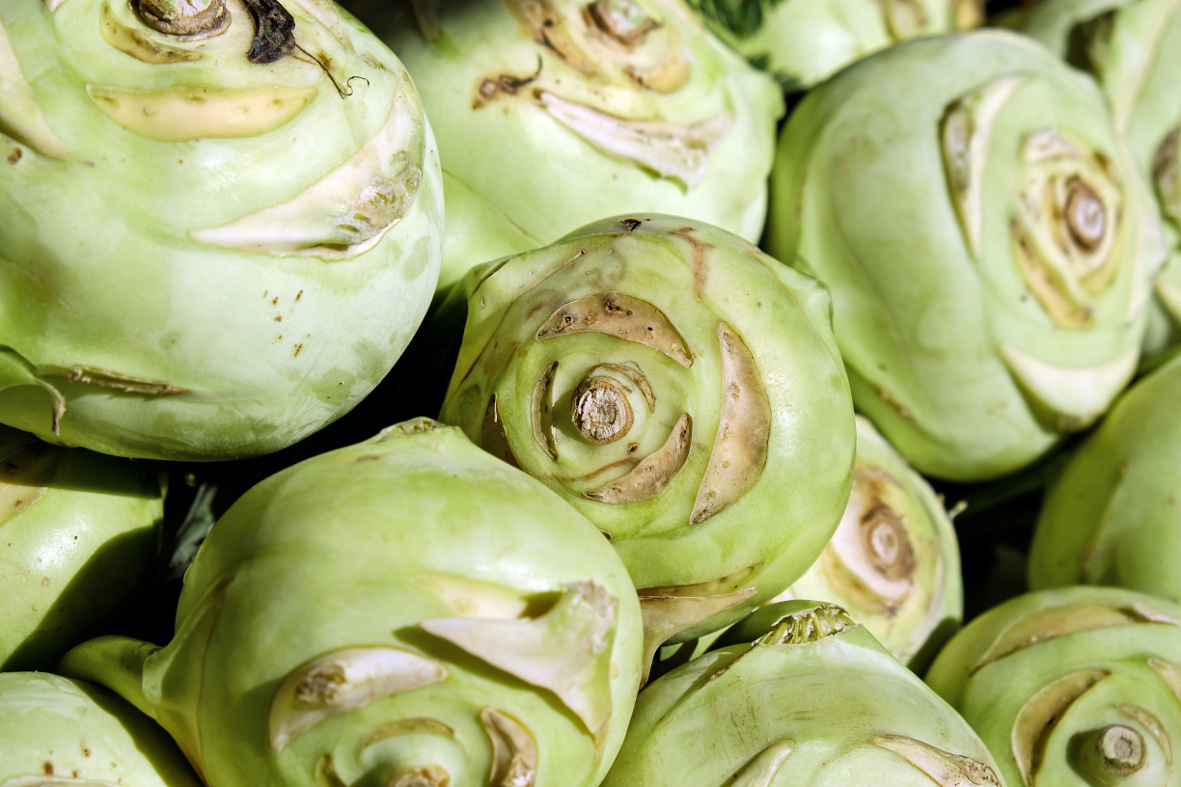
\includegraphics[width=3.94in]{kohlrabi-2266665-klein} 

}

\caption{Figure caption}\label{fig:koolrabi2}
\end{figure}

\hypertarget{h:formules}{%
\chapter{Equations}\label{h:formules}}

\hypertarget{inline-equations}{%
\section{Inline equations}\label{inline-equations}}

Inline equation fit within the paragraph. E.g.
\(P(y < Y|\theta) = \alpha\). This works OK with short equations. More
complex, taller equation will altered to minize their height,
e.g.~\(\bar{X} = \sum_{i = 1}^NX_i\). \(i = 1\) and \(N\) are placed
beside \(\sum\) instead of above it. This doesn't work with even taller
equations like breaks, e.g.~\(\frac{X}{Y}\). In this case the font size
is decreased. Complex equations like
\(\frac{\sum_{i = 1}^NX_i}{\frac{\sum_{j = 1}^NY_j}{N}}\) require a
larger interline distance. A stand alone equations is a better solution
for complex equations.

\hypertarget{stand-alone-equations}{%
\section{Stand alone equations}\label{stand-alone-equations}}

\[P(y < Y|\theta) = \alpha\]

\[\bar{X} = \sum_{i = 1}^NX_i\]

\[\frac{X}{Y}\]

\[\frac{\sum_{i = 1}^NX_i}{\frac{\sum_{j = 1}^NY_i}{N}}\]

\hypertarget{s:formule-nummer}{%
\section{Numberd equations}\label{s:formule-nummer}}

\begin{equation}
  \bar{X} = \sum_{i = 1}^NX_i
  \label{eq:som}
\end{equation}

\begin{equation}
  \frac{X}{Y}
\end{equation}

\begin{equation}
  \frac{\sum_{i = 1}^NX_i}{\frac{\sum_{j = 1}^NY_j}{N}}
\end{equation}

\hypertarget{citing-literature}{%
\chapter{Citing literature}\label{citing-literature}}

\hypertarget{inline-style}{%
\section{Inline style}\label{inline-style}}

\begin{itemize}
\tightlist
\item
  \protect\hyperlink{ref-BlauwdrukVleermuizen}{Onkelinx \emph{et al.}}
  (\protect\hyperlink{ref-BlauwdrukVleermuizen}{2014b})
\item
  (\protect\hyperlink{ref-BlauwdrukVleermuizen}{Onkelinx \emph{et al.},
  2014b})
\item
  (zie \protect\hyperlink{ref-BlauwdrukVleermuizen}{Onkelinx \emph{et
  al.}, 2014b}, hoofdstuk 1)
\item
  (\protect\hyperlink{ref-BlauwdrukVleermuizen}{Onkelinx \emph{et al.},
  2014b}, \protect\hyperlink{ref-Onkelinx2014a}{2014a})
\end{itemize}

\begin{description}
\tightlist
\item[book]
(\protect\hyperlink{ref-Agresti2002}{Agresti, 2002};
\protect\hyperlink{ref-BanerjeeEtal2003}{Banerjee \emph{et al.}, 2003};
\protect\hyperlink{ref-Bolker2008}{Bolker, 2008};
\protect\hyperlink{ref-book-a1e0}{Book, 2020};
\protect\hyperlink{ref-DiggleRibeiro2007}{Diggle \& Ribeiro, 2007};
\protect\hyperlink{ref-franklin_mapping_2009}{Franklin, 2009};
\protect\hyperlink{ref-Kish_1965}{Kish, 1965};
\protect\hyperlink{ref-ZuurEtal2009}{Zuur \emph{et al.}, 2009})
\item[chapter]
(\protect\hyperlink{ref-BlauwdrukVogels}{Anselin \emph{et al.}, 2014};
\protect\hyperlink{ref-Degraer2013a}{Degraer \emph{et al.}, 2013};
\protect\hyperlink{ref-BlauwdrukVleermuizen}{Onkelinx \emph{et al.},
2014b})
\item[proceedings]
(\protect\hyperlink{ref-Onkelinx2012}{Onkelinx \emph{et al.}, 2012},
\protect\hyperlink{ref-Onkelinx2014a}{2014a})
\item[article]
(\protect\hyperlink{ref-Amano2012}{Amano, 2012};
\protect\hyperlink{ref-VanderMijnsbrugge2005}{Vander Mijnsbrugge \&
Onkelinx, 2005}; \protect\hyperlink{ref-R-reshape}{Wickham, 2007};
\protect\hyperlink{ref-Yli-Viikari2007}{Yli-Viikari \emph{et al.},
2007})
\item[thesis]
(\protect\hyperlink{ref-MaStatThesis}{Onkelinx, 2009})
\item[software]
(\protect\hyperlink{ref-R-3.0.1}{R Core Team, 2013})
\end{description}

sans date:
\protect\hyperlink{ref-databank_ondergrond_vlaanderen_bepalen_nodate}{Databank
Ondergrond Vlaanderen}
(\protect\hyperlink{ref-databank_ondergrond_vlaanderen_bepalen_nodate}{s.~d.})

\hypertarget{code}{%
\chapter{Code}\label{code}}

\begin{Shaded}
\begin{Highlighting}[]
\CommentTok{\# logical}
\FunctionTok{c}\NormalTok{(}\ConstantTok{TRUE}\NormalTok{, }\ConstantTok{FALSE}\NormalTok{)}
\end{Highlighting}
\end{Shaded}

\begin{verbatim}
## [1]  TRUE FALSE
\end{verbatim}

\begin{Shaded}
\begin{Highlighting}[]
\CommentTok{\# integer}
\DecValTok{0}\SpecialCharTok{:}\DecValTok{1}
\end{Highlighting}
\end{Shaded}

\begin{verbatim}
## [1] 0 1
\end{verbatim}

\begin{Shaded}
\begin{Highlighting}[]
\CommentTok{\# numeric}
\FunctionTok{c}\NormalTok{(}\FloatTok{0.0}\NormalTok{, }\FloatTok{1.1}\NormalTok{)}
\end{Highlighting}
\end{Shaded}

\begin{verbatim}
## [1] 0.0 1.1
\end{verbatim}

\begin{Shaded}
\begin{Highlighting}[]
\CommentTok{\# scientific}
\FunctionTok{c}\NormalTok{(}\FloatTok{1e{-}10}\NormalTok{, }\FloatTok{1e10}\NormalTok{)}
\end{Highlighting}
\end{Shaded}

\begin{verbatim}
## [1] 1e-10 1e+10
\end{verbatim}

\begin{Shaded}
\begin{Highlighting}[]
\CommentTok{\# character}
\FunctionTok{c}\NormalTok{(}\StringTok{"Monday"}\NormalTok{, }\StringTok{"Tuesday"}\NormalTok{, }\StringTok{"Wednesday"}\NormalTok{)}
\end{Highlighting}
\end{Shaded}

\begin{verbatim}
## [1] "Monday"    "Tuesday"   "Wednesday"
\end{verbatim}

\begin{Shaded}
\begin{Highlighting}[]
\CommentTok{\# factor}
\FunctionTok{factor}\NormalTok{(}\FunctionTok{c}\NormalTok{(}\StringTok{"Monday"}\NormalTok{, }\StringTok{"Tuesday"}\NormalTok{, }\StringTok{"Wednesday"}\NormalTok{))}
\end{Highlighting}
\end{Shaded}

\begin{verbatim}
## [1] Monday    Tuesday   Wednesday
## Levels: Monday Tuesday Wednesday
\end{verbatim}

\begin{Shaded}
\begin{Highlighting}[]
\CommentTok{\# function}
\NormalTok{my\_fun }\OtherTok{\textless{}{-}} \ControlFlowTok{function}\NormalTok{(x)\{}
  \FunctionTok{cat}\NormalTok{(}\StringTok{"my function is"}\NormalTok{, x)}
\NormalTok{\}}
\CommentTok{\# data.frame}
\NormalTok{state }\OtherTok{\textless{}{-}} \FunctionTok{data.frame}\NormalTok{(}
  \AttributeTok{region =}\NormalTok{ state.region,}
  \AttributeTok{Division =}\NormalTok{ state.division,}
\NormalTok{  state.x77}
\NormalTok{)}
\CommentTok{\# function}
\FunctionTok{my\_fun}\NormalTok{(}\StringTok{"cool"}\NormalTok{)}
\end{Highlighting}
\end{Shaded}

\begin{verbatim}
## my function is cool
\end{verbatim}

\begin{Shaded}
\begin{Highlighting}[]
\CommentTok{\# boodschappen}
\FunctionTok{message}\NormalTok{(}\StringTok{"this is a message"}\NormalTok{)}
\end{Highlighting}
\end{Shaded}

\begin{verbatim}
## this is a message
\end{verbatim}

\begin{Shaded}
\begin{Highlighting}[]
\FunctionTok{warning}\NormalTok{(}\StringTok{"this is a warning"}\NormalTok{)}
\end{Highlighting}
\end{Shaded}

\begin{verbatim}
## Warning: this is a warning
\end{verbatim}

\begin{Shaded}
\begin{Highlighting}[]
\FunctionTok{stop}\NormalTok{(}\StringTok{"this is an error message"}\NormalTok{)}
\end{Highlighting}
\end{Shaded}

\begin{verbatim}
## Error in eval(expr, envir, enclos): this is an error message
\end{verbatim}

\begin{Shaded}
\begin{Highlighting}[]
\CommentTok{\# programma flow}
\ControlFlowTok{if}\NormalTok{ (}\FunctionTok{is.data.frame}\NormalTok{(state)) \{}
  \FunctionTok{summary}\NormalTok{(state)}
\NormalTok{\} }\ControlFlowTok{else}\NormalTok{ \{}
  \FunctionTok{stop}\NormalTok{(}\StringTok{"state is not a data.frame"}\NormalTok{)}
\NormalTok{\}}
\end{Highlighting}
\end{Shaded}

\begin{verbatim}
##            region                 Division    Population        Income       Illiteracy       Life.Exp    
##  Northeast    : 9   South Atlantic    : 8   Min.   :  365   Min.   :3098   Min.   :0.500   Min.   :67.96  
##  South        :16   Mountain          : 8   1st Qu.: 1080   1st Qu.:3993   1st Qu.:0.625   1st Qu.:70.12  
##  North Central:12   West North Central: 7   Median : 2838   Median :4519   Median :0.950   Median :70.67  
##  West         :13   New England       : 6   Mean   : 4246   Mean   :4436   Mean   :1.170   Mean   :70.88  
##                     East North Central: 5   3rd Qu.: 4968   3rd Qu.:4814   3rd Qu.:1.575   3rd Qu.:71.89  
##                     Pacific           : 5   Max.   :21198   Max.   :6315   Max.   :2.800   Max.   :73.60  
##                     (Other)           :11                                                                 
##      Murder          HS.Grad          Frost             Area       
##  Min.   : 1.400   Min.   :37.80   Min.   :  0.00   Min.   :  1049  
##  1st Qu.: 4.350   1st Qu.:48.05   1st Qu.: 66.25   1st Qu.: 36985  
##  Median : 6.850   Median :53.25   Median :114.50   Median : 54277  
##  Mean   : 7.378   Mean   :53.11   Mean   :104.46   Mean   : 70736  
##  3rd Qu.:10.675   3rd Qu.:59.15   3rd Qu.:139.75   3rd Qu.: 81163  
##  Max.   :15.100   Max.   :67.30   Max.   :188.00   Max.   :566432  
## 
\end{verbatim}

\begin{Shaded}
\begin{Highlighting}[]
\ControlFlowTok{for}\NormalTok{ (i }\ControlFlowTok{in} \DecValTok{1}\SpecialCharTok{:}\DecValTok{5}\NormalTok{) \{}
  \FunctionTok{cat}\NormalTok{(}\StringTok{"i ="}\NormalTok{, i, }\StringTok{"}\SpecialCharTok{\textbackslash{}n}\StringTok{"}\NormalTok{)}
\NormalTok{\}}
\end{Highlighting}
\end{Shaded}

\begin{verbatim}
## i = 1 
## i = 2 
## i = 3 
## i = 4 
## i = 5
\end{verbatim}

\hypertarget{figures}{%
\chapter{Figures}\label{figures}}

\hypertarget{inline-figure}{%
\section{Inline figure}\label{inline-figure}}

\begin{Shaded}
\begin{Highlighting}[]
\FunctionTok{ggplot}\NormalTok{(}
\NormalTok{  mtcars, }
  \FunctionTok{aes}\NormalTok{(}\AttributeTok{x =}\NormalTok{ wt, }\AttributeTok{y =}\NormalTok{ mpg, }\AttributeTok{colour =} \FunctionTok{factor}\NormalTok{(cyl), }\AttributeTok{fill =} \FunctionTok{factor}\NormalTok{(cyl))}
\NormalTok{) }\SpecialCharTok{+}
  \FunctionTok{geom\_point}\NormalTok{() }\SpecialCharTok{+} 
  \FunctionTok{geom\_smooth}\NormalTok{(}\AttributeTok{method =} \StringTok{"lm"}\NormalTok{)}
\end{Highlighting}
\end{Shaded}

\begin{verbatim}
## `geom_smooth()` using formula 'y ~ x'
\end{verbatim}

\begin{center}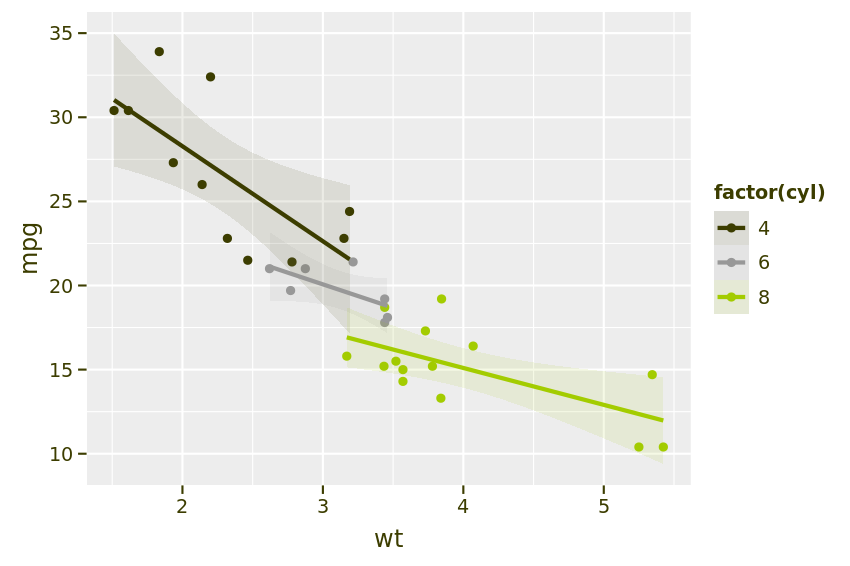
\includegraphics{flandre_rapport_files/figure-latex/gg-mtcars-1} \end{center}

\hypertarget{floating-figure}{%
\section{Floating figure}\label{floating-figure}}

\begin{Shaded}
\begin{Highlighting}[]
\FunctionTok{ggplot}\NormalTok{(esoph, }\FunctionTok{aes}\NormalTok{(}\AttributeTok{x =}\NormalTok{ ncases }\SpecialCharTok{/}\NormalTok{ (ncases }\SpecialCharTok{+}\NormalTok{ ncontrols))) }\SpecialCharTok{+} 
  \FunctionTok{geom\_histogram}\NormalTok{() }\SpecialCharTok{+} 
  \FunctionTok{facet\_wrap}\NormalTok{(}\SpecialCharTok{\textasciitilde{}}\NormalTok{agegp, }\AttributeTok{scales =} \StringTok{"free"}\NormalTok{)}
\end{Highlighting}
\end{Shaded}

\begin{figure}

{\centering 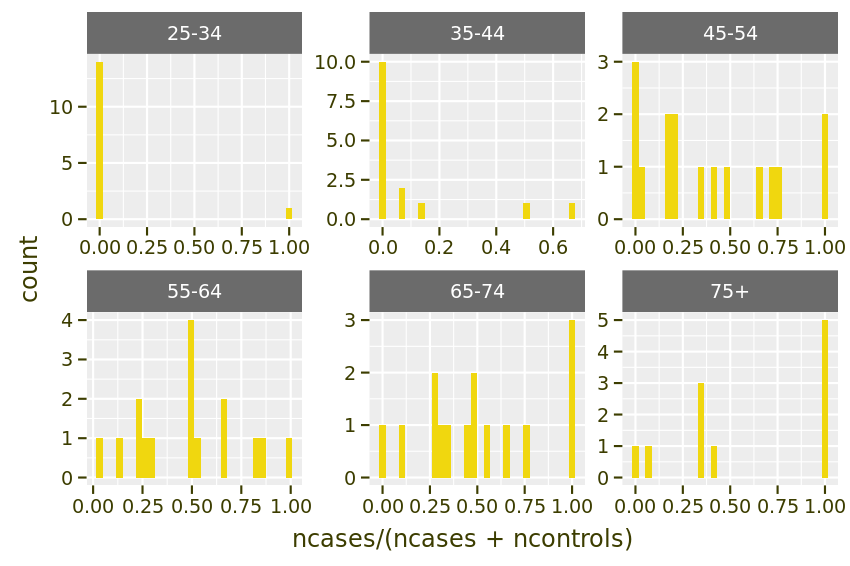
\includegraphics{flandre_rapport_files/figure-latex/movie-1} 

}

\caption{Distribution of esophageal cancer in Ille-et-Villaine, France.}\label{fig:movie}
\end{figure}

\begin{Shaded}
\begin{Highlighting}[]
\FunctionTok{ggplot}\NormalTok{(diamonds, }\FunctionTok{aes}\NormalTok{(}\AttributeTok{x =}\NormalTok{ price, }\AttributeTok{fill =}\NormalTok{ cut)) }\SpecialCharTok{+} 
  \FunctionTok{geom\_histogram}\NormalTok{()}
\end{Highlighting}
\end{Shaded}

\begin{figure}

{\centering 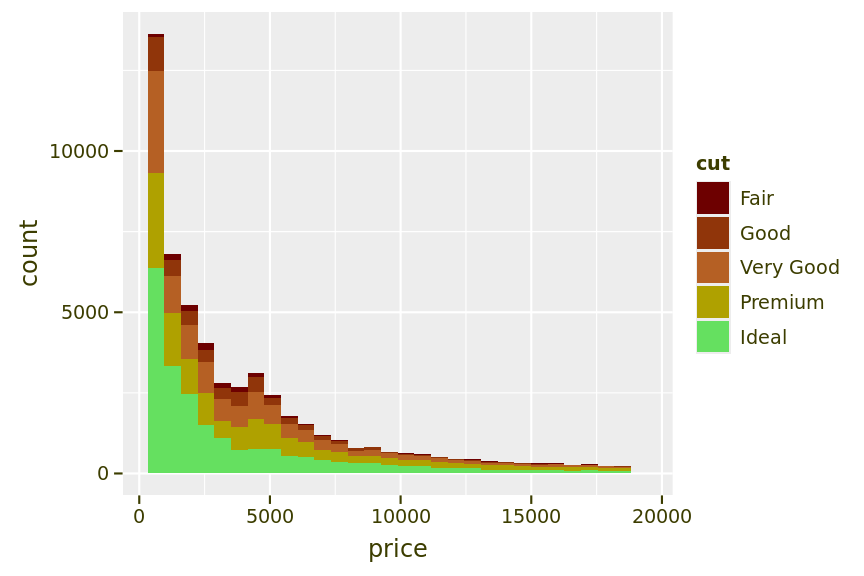
\includegraphics{flandre_rapport_files/figure-latex/diamond-1} 

}

\caption{Histrogram of the price of diamonds}\label{fig:diamond}
\end{figure}

\begin{Shaded}
\begin{Highlighting}[]
\FunctionTok{ggplot}\NormalTok{(}
\NormalTok{  mtcars, }
  \FunctionTok{aes}\NormalTok{(}\AttributeTok{x =}\NormalTok{ wt, }\AttributeTok{y =}\NormalTok{ mpg, }\AttributeTok{colour =} \FunctionTok{factor}\NormalTok{(cyl), }\AttributeTok{fill =} \FunctionTok{factor}\NormalTok{(cyl))}
\NormalTok{) }\SpecialCharTok{+}
  \FunctionTok{geom\_point}\NormalTok{() }\SpecialCharTok{+} 
  \FunctionTok{geom\_smooth}\NormalTok{(}\AttributeTok{method =} \StringTok{"lm"}\NormalTok{) }
\end{Highlighting}
\end{Shaded}

\begin{verbatim}
## `geom_smooth()` using formula 'y ~ x'
\end{verbatim}

\begin{figure}

{\centering 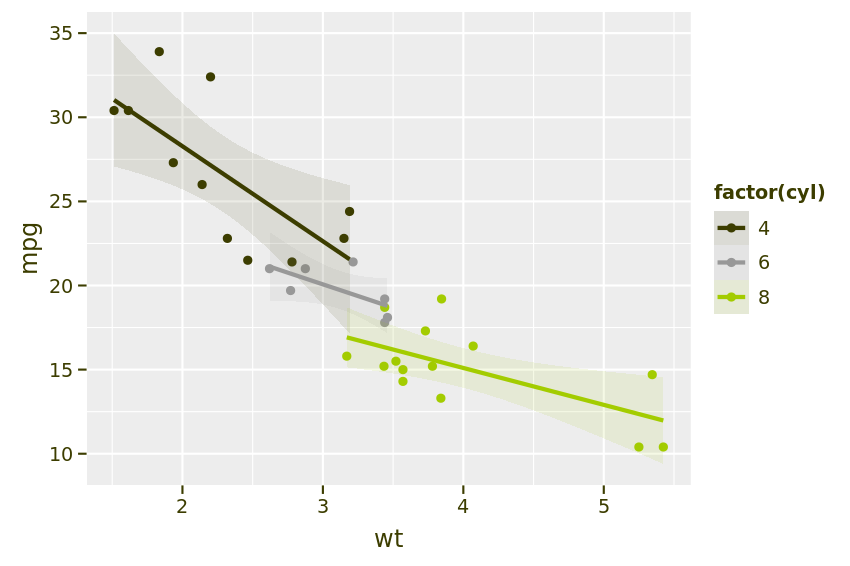
\includegraphics{flandre_rapport_files/figure-latex/gg-mtcars1-1} 

}

\caption{Fuel consumption for 1974 cars in miles per gallon.}\label{fig:gg-mtcars1}
\end{figure}

\hypertarget{tables-1}{%
\chapter{Tables}\label{tables-1}}

\begin{Shaded}
\begin{Highlighting}[]
\CommentTok{\# functions to generate tables}
\NormalTok{digit\_table }\OtherTok{\textless{}{-}} \ControlFlowTok{function}\NormalTok{(}\AttributeTok{rows =} \DecValTok{20}\NormalTok{, }\AttributeTok{cols =} \DecValTok{10}\NormalTok{) \{}
  \FunctionTok{data.frame}\NormalTok{(}
    \FunctionTok{matrix}\NormalTok{(}
      \FunctionTok{rnorm}\NormalTok{(rows }\SpecialCharTok{*}\NormalTok{ cols),}
      \AttributeTok{nrow =}\NormalTok{ rows,}
      \AttributeTok{ncol =}\NormalTok{ cols}
\NormalTok{    ),}
    \AttributeTok{row.names =} \FunctionTok{paste}\NormalTok{(}\StringTok{"row"}\NormalTok{, }\FunctionTok{seq\_len}\NormalTok{(rows))}
\NormalTok{  )}
\NormalTok{\}}
\NormalTok{random\_word }\OtherTok{\textless{}{-}} \ControlFlowTok{function}\NormalTok{(}\AttributeTok{n\_letters =} \DecValTok{5}\NormalTok{)\{}
  \FunctionTok{paste}\NormalTok{(}
    \FunctionTok{sample}\NormalTok{(letters, }\AttributeTok{size =}\NormalTok{ n\_letters, }\AttributeTok{replace =} \ConstantTok{TRUE}\NormalTok{),}
    \AttributeTok{collapse =} \StringTok{""}
\NormalTok{  )}
\NormalTok{\}}
\NormalTok{random\_sentence }\OtherTok{\textless{}{-}} \ControlFlowTok{function}\NormalTok{(}\AttributeTok{words =} \DecValTok{10}\NormalTok{, }\AttributeTok{n\_letters =} \DecValTok{10}\NormalTok{)\{}
  \FunctionTok{paste}\NormalTok{(}
    \FunctionTok{sapply}\NormalTok{(}
      \FunctionTok{rpois}\NormalTok{(words, n\_letters), }
      \AttributeTok{FUN =}\NormalTok{ random\_word}
\NormalTok{    ),}
    \AttributeTok{collapse =} \StringTok{" "}
\NormalTok{  )}
\NormalTok{\}}
\NormalTok{text\_table }\OtherTok{\textless{}{-}} \ControlFlowTok{function}\NormalTok{(}\AttributeTok{rows =} \DecValTok{20}\NormalTok{, }\AttributeTok{cols =} \DecValTok{10}\NormalTok{, }\AttributeTok{words =} \DecValTok{10}\NormalTok{, }\AttributeTok{n\_letters =} \DecValTok{5}\NormalTok{)\{}
\NormalTok{  x }\OtherTok{\textless{}{-}} \FunctionTok{data.frame}\NormalTok{(}
    \FunctionTok{matrix}\NormalTok{(}
      \FunctionTok{sapply}\NormalTok{(}
        \FunctionTok{rpois}\NormalTok{(rows }\SpecialCharTok{*}\NormalTok{ cols, }\AttributeTok{lambda =}\NormalTok{ words), }
\NormalTok{        random\_sentence,}
\NormalTok{        n\_letters}
\NormalTok{      ),}
      \AttributeTok{nrow =}\NormalTok{ rows,}
      \AttributeTok{ncol =}\NormalTok{ cols}
\NormalTok{    )}
\NormalTok{  )}
  \FunctionTok{colnames}\NormalTok{(x) }\OtherTok{\textless{}{-}} \FunctionTok{head}\NormalTok{(LETTERS, cols)}
  \FunctionTok{return}\NormalTok{(x)}
\NormalTok{\}}
\NormalTok{generate\_table }\OtherTok{\textless{}{-}} \ControlFlowTok{function}\NormalTok{(}\AttributeTok{rows =} \DecValTok{20}\NormalTok{, }\AttributeTok{cols =} \FunctionTok{c}\NormalTok{(}\DecValTok{5}\NormalTok{, }\DecValTok{5}\NormalTok{), }\AttributeTok{words =} \DecValTok{10}\NormalTok{, }\AttributeTok{n\_letters =} \DecValTok{5}\NormalTok{)\{}
  \FunctionTok{cbind}\NormalTok{(}
    \FunctionTok{digit\_table}\NormalTok{(}\AttributeTok{rows =}\NormalTok{ rows, }\AttributeTok{cols =}\NormalTok{ cols[}\DecValTok{1}\NormalTok{]),}
    \FunctionTok{text\_table}\NormalTok{(}
      \AttributeTok{rows =}\NormalTok{ rows, }\AttributeTok{cols =}\NormalTok{ cols[}\DecValTok{2}\NormalTok{], }\AttributeTok{words =}\NormalTok{ words, }\AttributeTok{n\_letters =}\NormalTok{ n\_letters}
\NormalTok{    )}
\NormalTok{  )}
\NormalTok{\}}
\end{Highlighting}
\end{Shaded}

\hypertarget{kable}{%
\section{\texorpdfstring{\texttt{kable()}}{kable()}}\label{kable}}

\begin{Shaded}
\begin{Highlighting}[]
\FunctionTok{kable}\NormalTok{(}
  \FunctionTok{generate\_table}\NormalTok{(}\DecValTok{50}\NormalTok{, }\FunctionTok{c}\NormalTok{(}\DecValTok{4}\NormalTok{, }\DecValTok{2}\NormalTok{), }\DecValTok{4}\NormalTok{, }\DecValTok{4}\NormalTok{), }
  \AttributeTok{caption =} \StringTok{"Default \textasciigrave{}kable()\textasciigrave{} output."}
\NormalTok{)}
\end{Highlighting}
\end{Shaded}

\begin{table}

\caption{\label{tab:kable}Default `kable()` output.}
\centering
\begin{tabular}[t]{l|r|r|r|r|l|l}
\hline
  & X1 & X2 & X3 & X4 & A & B\\
\hline
row 1 & 0.4144963 & -0.6300042 & 0.2878449 & -0.6749138 & xlkxl ifkj & relkxf vridj wm yoahjvxyiyz crekxd iqqvs lvp lhtzv\\
\hline
row 2 & 0.0408233 & 1.1605534 & -0.5827246 & 0.3559498 & lhhznp ywhqq wd p lrdcv ovsc & mxgb emyurgez hnnfu kwpt t zyygcc\\
\hline
row 3 & 1.4690982 & 1.4515004 & -0.2419918 & -1.0759037 & ggpzilj dmy e buux & hy xcpq ufqlu\\
\hline
row 4 & -0.3475795 & 0.9727659 & -0.6215156 & 0.1974737 & nkc kjbk kf nmpxe aoi uauovoiuer fth trkgj ot brbp & ybn opp bceipv wm\\
\hline
row 5 & -1.2347692 & 1.4897325 & 0.0754181 & 1.3277529 & hihv suohm & stuuizz v fedwx uxetsoq\\
\hline
row 6 & -1.0499842 & -1.5119097 & -0.6509891 & 0.8173166 & ezr jhl inhb abcj gkw & lqlblnn zm devdtu bolw elvnk\\
\hline
row 7 & -1.1937549 & 0.5193834 & -0.5654466 & 1.6603580 & vu batko kp ojcig qtdjxhrqk aus & zf aujlu cx\\
\hline
row 8 & -0.0610155 & -0.1646181 & -0.5101061 & -0.1504200 & botg poy & wifuoyy gqnvyqxutqs\\
\hline
row 9 & 0.7582549 & -0.5499047 & -1.5756268 & -0.6216659 & gf ofuzg pdh kafbuv opet glqb & syfglprf hwi hz\\
\hline
row 10 & 0.7663292 & -2.6102884 & 1.7162299 & -1.3776557 & kzjn tnhf p heihbv kzus mllel & eetk gzw lg babz mbd\\
\hline
row 11 & 0.2421094 & 1.2109279 & -1.2543723 & 1.1352409 & mut tpks ktjdr & mfmj wog hqctzu ukz hwy\\
\hline
row 12 & 0.8234555 & -0.8712454 & -1.2053205 & -0.3004313 & vta & wehf ztw f xkb\\
\hline
row 13 & 0.4469607 & 0.4440394 & 1.2629634 & 0.7062932 & ybag yu wg & ly gyyj evrztj\\
\hline
row 14 & -1.0046833 & -0.2129330 & -0.1582419 & 0.8761494 & snodj n ragl & cmynm aaaods rycatt ro\\
\hline
row 15 & -0.9464531 & -0.7638588 & -0.3622425 & -1.3209908 & nqdjst mzqnr oznzzx aqp & kobgbcoqn beftj hkr zhdxbufl\\
\hline
row 16 & 0.8054786 & 0.4609743 & 0.2102750 & -1.2389517 & jyq vlb nxy & wox\\
\hline
row 17 & 0.2841325 & 1.2643887 & 0.9618151 & 0.2694317 & ymo asdpve de & cqoc jrwbl  vipujealu xnepnj\\
\hline
row 18 & 0.3773189 & -2.3015523 & -0.3454738 & 1.2980847 & mt & vmj ubrzvm frq o\\
\hline
row 19 & 1.0661467 & -0.8339385 & -0.9408881 & -1.3176954 & pnnfh y sshyiv qkgf tkvstwf kz & mohvm wae\\
\hline
row 20 & 0.8195030 & -0.4432494 & -0.8994477 & -1.0392347 & zcme & drxhi  gruz gltwlx icm hm fqkb\\
\hline
row 21 & -0.1962719 & -1.0100966 & -2.0516981 & 0.3008718 & zubwso oerzuaxi flkqjg & brf foqsipesw ktai xrsy\\
\hline
row 22 & -0.1564035 & 0.0599580 & -1.8130683 & 0.3020121 & mnkc ampsxz ppbm cquh eup lfvlgz & ie uzad uogw wvv es wv nwajim vm\\
\hline
row 23 & 0.4363182 & 0.1989392 & 0.6615051 & -1.6867486 & qzexibx df cyvd & drgtonmgh i v\\
\hline
row 24 & -0.5747251 & -0.9975262 & 0.4136543 & 0.4108156 & zix hhwbi q cta pfoe & dx hsud jjrfqav\\
\hline
row 25 & 0.6790750 & -0.0505454 & -0.6506578 & 0.9433994 & umtwo iuh fkkvutc & gtblb ti hlw ig obfhqgb bmygmq\\
\hline
row 26 & -1.6305303 & 0.3377164 & -1.5277428 & -1.6393180 & syqsjn q bc & vlil drpgf dsrz usvfnj qnrqs upscxnm kg si kgfdoeq\\
\hline
row 27 & 1.0331155 & -0.0525841 & 0.6309764 & -0.5558357 & l ikwk hy mx kft xn ht doon mtfhe kzh & erar cwe cmfg\\
\hline
row 28 & 1.5279120 & -0.0473316 & 0.5695529 & 3.0694315 & ys f ou ewdt & gexqk rcbm cfsj\\
\hline
row 29 & 1.9878485 & 1.3378993 & 0.0927983 & -0.8932157 & dmumhj & osw zizd  accapt\\
\hline
row 30 & 0.4034466 & -0.7754286 & 1.9028730 & 1.4746035 & wubxor vrdzsp ohp & pma rtnuh fs oq uhez\\
\hline
row 31 & 0.5855315 & 0.3785690 & 1.8400715 & 0.5143470 & osfly rae ucm suscz j & d th tcpy td\\
\hline
row 32 & 1.0246717 & 1.2296627 & -0.0365756 & -0.5290351 & afji tv & uyx lzzmdx ozj gvlmu\\
\hline
row 33 & -0.9315820 & 0.3947289 & 0.0876284 & 3.5389638 & mvq xup zjxkc uomhugp & ezhr xmzvacr ytce\\
\hline
row 34 & 0.5041985 & 0.3417828 & -0.1843824 & -1.0550961 & jqzwk fled pa qu & vaw r znth gu\\
\hline
row 35 & 1.1539391 & 0.8625262 & 1.7148065 & 0.8296601 & orgin aee ezo wsiqmcqp & bv v m natlj fhktz tnuxz\\
\hline
row 36 & 1.0685628 & -0.4316871 & 1.0360977 & -0.1715012 & t rshk al gr lbw & gbyjtre mrk bamskn\\
\hline
row 37 & 0.9436128 & -2.2012354 & 0.9637120 & 0.5170063 & tla gqi eixvwue & ex bx pvkom\\
\hline
row 38 & -0.1488094 & -0.9683051 & -0.5117687 & -1.8291550 & u eath rjuis ik ijp qjroy es & osfylqsipm lr\\
\hline
row 39 & 0.9318746 & 0.0084124 & -0.6068602 & -1.1889430 & ytccr rypuplfr itx xys snahqdbd & ln ag xdhp ypaf\\
\hline
row 40 & -2.3850909 & -0.6384056 & -1.1933902 & 0.6901838 & pzb yk ovnvtit la & qdunmv d xu xm\\
\hline
row 41 & -0.2852951 & 1.7175429 & -0.1733689 & -0.0204748 & fo & idfqa dz coxxvao bmr ms um rbox stt\\
\hline
row 42 & 0.7186323 & -1.3137459 & 2.0967799 & 0.3521966 & zjg vwt nmgdo ufl & khek tvwui mhuv wyi\\
\hline
row 43 & 0.0490366 & -0.6721416 & 0.1644419 & 0.8682230 & zhxjbjr dnoe tes kzh bqqd & vvb grolje  zwze\\
\hline
row 44 & -0.7116361 & 1.4158066 & 0.4899534 & 0.0578012 & pl & jip jzh w dv zcdi\\
\hline
row 45 & 0.8444659 & 0.9689673 & 0.9425010 & 0.8847459 & lxvn cfg pwn & hbpwch alupi uoq dqw txslrav ovmp\\
\hline
row 46 & -0.4775350 & -0.9768303 & -0.7990541 & -1.2692668 & uhpakcfs jk qols & dya wdwmj\\
\hline
row 47 & 0.2603214 & -0.6154838 & 1.1609327 & 0.7556511 & f  mbp & eov\\
\hline
row 48 & 0.3458669 & 1.0546258 & 0.7270006 & -0.1439999 & s z aqinia & cktiw xtxws\\
\hline
row 49 & 1.7851982 & 0.0105253 & 0.8343401 & 0.4860110 & ixcd gqbtevl myleupfefi lorbhs olckuhsbn & fyem hewdtige\\
\hline
row 50 & 1.0612401 & 0.2648408 & 1.3074218 & 1.3492607 & tr fb izq & joftbt ynwizg\\
\hline
\end{tabular}
\end{table}

\begin{Shaded}
\begin{Highlighting}[]
\FunctionTok{kable}\NormalTok{(}
  \FunctionTok{generate\_table}\NormalTok{(}\DecValTok{20}\NormalTok{, }\FunctionTok{c}\NormalTok{(}\DecValTok{4}\NormalTok{, }\DecValTok{3}\NormalTok{), }\DecValTok{5}\NormalTok{, }\DecValTok{4}\NormalTok{), }
  \AttributeTok{digits =} \DecValTok{2}\NormalTok{,}
  \AttributeTok{format =} \StringTok{"markdown"}
\NormalTok{)}
\end{Highlighting}
\end{Shaded}

\begin{longtable}[]{@{}
  >{\raggedright\arraybackslash}p{(\columnwidth - 14\tabcolsep) * \real{0.04}}
  >{\raggedleft\arraybackslash}p{(\columnwidth - 14\tabcolsep) * \real{0.03}}
  >{\raggedleft\arraybackslash}p{(\columnwidth - 14\tabcolsep) * \real{0.03}}
  >{\raggedleft\arraybackslash}p{(\columnwidth - 14\tabcolsep) * \real{0.03}}
  >{\raggedleft\arraybackslash}p{(\columnwidth - 14\tabcolsep) * \real{0.03}}
  >{\raggedright\arraybackslash}p{(\columnwidth - 14\tabcolsep) * \real{0.25}}
  >{\raggedright\arraybackslash}p{(\columnwidth - 14\tabcolsep) * \real{0.36}}
  >{\raggedright\arraybackslash}p{(\columnwidth - 14\tabcolsep) * \real{0.23}}@{}}
\toprule
\begin{minipage}[b]{\linewidth}\raggedright
\end{minipage} & \begin{minipage}[b]{\linewidth}\raggedleft
X1
\end{minipage} & \begin{minipage}[b]{\linewidth}\raggedleft
X2
\end{minipage} & \begin{minipage}[b]{\linewidth}\raggedleft
X3
\end{minipage} & \begin{minipage}[b]{\linewidth}\raggedleft
X4
\end{minipage} & \begin{minipage}[b]{\linewidth}\raggedright
A
\end{minipage} & \begin{minipage}[b]{\linewidth}\raggedright
B
\end{minipage} & \begin{minipage}[b]{\linewidth}\raggedright
C
\end{minipage} \\
\midrule
\endhead
row 1 & 0.55 & 0.87 & -0.76 & -0.88 & wt pk dtsyeb & fwke jinih & qzgps
ypfnn akzt rbg hdazp xnjyf ez bzah \\
row 2 & 0.88 & -0.50 & 0.10 & 0.44 & wdhlz ocw & a zzuk qop n gdd bvk &
fct vhi \\
row 3 & 0.11 & -0.95 & -0.84 & 0.51 & jgt dvtaugfur & abz fth safjc &
wialvo cwwhf ar kftxgtvpm \\
row 4 & 0.48 & -0.29 & -0.94 & -1.62 & & ufcy sasryb zff wemgtml e &
vmevro vtuo ybhi yqnoa secg tzv nlap kumta \\
row 5 & -0.72 & -0.39 & -0.06 & 1.23 & utpfd qs mlif & engsgb bsd hkqkg
g g bvvx & qimi amxixdhvas waa aqobx kkyqlffw b \\
row 6 & -1.11 & 0.16 & 0.59 & -0.29 & urprtkq l gofyvm qnrx vnfbg lig &
pfs xbpay gwxc wbh vzqyw cctspwis & puxgjxeo xgylnx pls yggnb noa
vzju \\
row 7 & -0.25 & -0.63 & 0.53 & 0.32 & ttj eizfx x jqlvx p mlciy & rodzb
n cfm & tzu ypdq zg iplr \\
row 8 & -1.16 & 1.29 & -0.57 & -1.98 & lps ycrabi ybbffnniv zxrgw mcc &
wdce hjotb xs cppeh co tvcdvkx oibzbsbh msb & yq unjk hie fwb mz hd ns
myd \\
row 9 & -0.22 & -0.33 & 0.83 & -1.47 & g jxrz kcvbocyo h & qbfe r
chmwwiuim xybklk & jugjj iqabo doafj \\
row 10 & -0.71 & -0.25 & 0.18 & -0.12 & aih zxtern beracgk gw if djgmfh
& pfc xgc ynir nsbzme kchasmaau ijbj & jh xfnuc nbwqfi \\
row 11 & 0.61 & -0.47 & 1.62 & -0.72 & gswmah ka yoflrmnk vhhcst xmkeyq
& ohto zut ctojnrk bzahn q & tqjv znq wm dwb \\
row 12 & 0.70 & -1.85 & -0.55 & 0.60 & fzvavvrrn & blxjn rvdz z ucf nwnn
& wa zugu bjnhf \\
row 13 & -0.86 & 1.56 & -1.15 & -0.51 & ardsx hib wvgc bwtoily ovadr &
memak jst xj qcbuvxhm wwmrh & vclti jsbkm briogo h zj gp njmuzq \\
row 14 & -0.83 & 0.92 & -0.37 & 1.69 & tnionxhk & pvz gihrld hpj dze
pcxk mivjrl kijkduy fwm bgwmpwyi rnoxbei pgrgvl & oxcxp gyqd syevbkj
jkxym drnt \\
row 15 & -1.33 & -1.43 & -0.15 & 1.56 & pu kv uta kgxw iw qzi wcy c
gvlymf zzjzvus egl & of hbn ciewf saa at l & wbwxevgh ogpgs lhgpsl \\
row 16 & 0.80 & -1.30 & 0.60 & -1.38 & vnhh tc & ice nun tlaot ebhno pf
zfrcb & ox nttsaab rmpnoo \\
row 17 & 0.08 & 2.85 & -1.05 & 0.18 & kjj hkod jtkku xslfwbuqr & & fivs
yksj t \\
row 18 & 1.46 & -1.29 & -0.35 & -0.74 & fu rhpu t xr sxrdd & wk got
cavcmyq qmka flcswa jwf & mccagdnx rugmox zngs \\
row 19 & -0.64 & 1.17 & -1.72 & 1.04 & zeplx no twbzcj gdchqsy hkisg
dvvr dvc & oyrcz rezmyy cxym wxfme & l halg hxbr sbu cjhv \\
row 20 & -0.93 & 0.77 & 0.59 & 0.92 & wi pzuo r & lfcuwe jsdm hk ekygw &
jyaeyw kaqov ds veib hjozz \\
\bottomrule
\end{longtable}

\begin{Shaded}
\begin{Highlighting}[]
\FunctionTok{kable}\NormalTok{(}
  \FunctionTok{generate\_table}\NormalTok{(}\DecValTok{50}\NormalTok{, }\FunctionTok{c}\NormalTok{(}\DecValTok{3}\NormalTok{, }\DecValTok{1}\NormalTok{), }\DecValTok{4}\NormalTok{, }\DecValTok{4}\NormalTok{), }
  \AttributeTok{digits =} \DecValTok{3}\NormalTok{,}
  \AttributeTok{caption =} \StringTok{"pandoc output van \textasciigrave{}kable()\textasciigrave{}"}\NormalTok{,}
  \AttributeTok{format =} \StringTok{"pandoc"}
\NormalTok{)}
\end{Highlighting}
\end{Shaded}

\begin{longtable}[]{@{}lrrrl@{}}
\caption{\label{tab:kable-pandoc}pandoc output van
\texttt{kable()}}\tabularnewline
\toprule
& X1 & X2 & X3 & A \\
\midrule
\endfirsthead
\toprule
& X1 & X2 & X3 & A \\
\midrule
\endhead
row 1 & 1.183 & 1.394 & -1.666 & msxd krs rfklf wg imi \\
row 2 & -0.460 & -1.568 & 0.040 & rcysu easft \\
row 3 & -0.378 & -2.140 & 0.659 & fvf hpkay vptglt eqjch uh \\
row 4 & -0.911 & -0.867 & 0.334 & qrng vp dlwb chma \\
row 5 & -0.103 & 2.510 & -0.563 & u ne m odzix djmib jcik \\
row 6 & -0.368 & -0.096 & -1.021 & tkgyq hfeoco vpunklra l gjznsy \\
row 7 & -0.186 & -0.450 & 1.262 & jzawpp tit pkqf de \\
row 8 & 0.245 & 2.181 & -1.607 & ksh pwmgjoig g cktsf udmpc towiyxcq
in \\
row 9 & 0.916 & 0.312 & 1.166 & qxkvoqq jcymtma mcrpa \\
row 10 & -0.364 & 0.278 & -0.486 & r jxp n b wion \\
row 11 & -0.046 & -1.187 & -0.003 & kekszh xii bzhxbi uktveexjf
bkmtnnbnze lvf \\
row 12 & -0.613 & -1.149 & -0.152 & cpf ut qndcvi lsqtrrs bjmv \\
row 13 & 0.839 & -1.212 & -1.432 & zha \\
row 14 & 0.031 & 0.565 & -0.519 & xv \\
row 15 & -0.497 & -0.876 & -0.152 & yui ktdoao \\
row 16 & -1.387 & -1.089 & -1.973 & grmwfij affpk juzitx xsjjg xgcfl \\
row 17 & -0.617 & -1.015 & -0.169 & odl a \\
row 18 & 0.103 & 0.122 & 1.182 & mcc tidxefv xdobllrg \\
row 19 & -0.094 & 0.972 & -0.484 & vka lnvb wjcz hbq \\
row 20 & 0.058 & 0.201 & -1.202 & c eruj \\
row 21 & -0.226 & 1.358 & 0.163 & ftbhzapq iz fpnl t \\
row 22 & 0.528 & 0.664 & -0.860 & r boxp py wjil srpjtczv tos noxrfrmm
apyqtjmm \\
row 23 & 0.901 & 0.174 & 0.121 & hfydv tczfgp ovun hak srainp pzq xfv
dxm rhv \\
row 24 & 0.270 & 1.101 & -0.845 & oltt fhz e \\
row 25 & -0.925 & 0.838 & 0.767 & gm afevej ez no jpba pcp \\
row 26 & -0.991 & -0.106 & -0.667 & xu mrymhq iuj uhcbqx gehyu qjh yx \\
row 27 & -0.144 & 0.677 & 1.645 & dj lboye uaf ensku valc fypojqgs \\
row 28 & -0.381 & 0.545 & 0.584 & cyllgczt rc \\
row 29 & 0.069 & -0.205 & -2.233 & ykrbyp vzqbo wddp \\
row 30 & -2.463 & 0.592 & -0.274 & aahou odoagpwqs wett pviy xlloc \\
row 31 & 0.523 & -0.793 & 0.116 & m \\
row 32 & 0.124 & 0.168 & -0.461 & erl jhvt jtj \\
row 33 & -0.044 & -1.507 & -0.933 & knb r d krd npq \\
row 34 & -0.844 & -1.946 & -0.089 & nsbxz usmxi ujpf atnupvoj m s \\
row 35 & -1.334 & -0.164 & -0.631 & itx bec ry \\
row 36 & -0.138 & -0.006 & -1.301 & sx mkak fqh \\
row 37 & 0.082 & -0.669 & 0.654 & n \\
row 38 & 0.760 & -0.975 & 0.514 & qd pim uufd \\
row 39 & -1.065 & -1.178 & 0.287 & xvnuf yboa g vclyj wtrksfzw ety \\
row 40 & 0.391 & -0.149 & 0.557 & kak oobiz nxz gfpqbpg oqpxms \\
row 41 & -1.269 & -0.065 & 0.327 & e vb glq n ina \\
row 42 & -1.464 & 0.270 & 1.001 & qvv bzi yw \\
row 43 & -2.036 & -1.386 & -0.090 & p bhxkc folx zfmlii cfxomcnw ljpokx
xfgs hp amoglj \\
row 44 & -0.455 & -0.610 & -0.332 & e vhi ujn neap reru \\
row 45 & 0.644 & 2.013 & -1.454 & lrnhmnuz eix axowv diwev vutflz \\
row 46 & 0.481 & -1.059 & 1.029 & azlf icz hg wpcab \\
row 47 & -0.027 & -0.721 & -1.166 & utlkcrhthh qfq nsurh bkpabgng \\
row 48 & 0.299 & 0.812 & 0.061 & glrac \\
row 49 & 0.535 & 0.123 & -0.619 & gvptfwuay vd nuu bu txfpx \\
row 50 & -0.194 & 0.346 & 2.270 & vurrt dr o b botn qevnwluc \\
\bottomrule
\end{longtable}

\chapter*{\bibname}
\addcontentsline{toc}{chapter}{\bibname}
\hypertarget{refs}{}

\begin{CSLReferences}{1}{0}

\leavevmode\vadjust pre{\hypertarget{ref-Agresti2002}{}}%
Agresti A. (2002). {Categorical Data Analysis}. John Wiley {and} Sons,
Hoboken, New Jersey.

\leavevmode\vadjust pre{\hypertarget{ref-Amano2012}{}}%
Amano T. (2012). {Unravelling the dynamics of organisms in a changing
world using ecological modelling}. Ecological Research 27 (3): 495‑507.
\url{https://doi.org/10.1007/s11284-012-0928-6}.

\leavevmode\vadjust pre{\hypertarget{ref-BlauwdrukVogels}{}}%
Anselin A., Devos K. \& Vermeersch G. (2014). {Blauwdruk Vogels}. In: De
Knijf G., Westra T., Onkelinx T., Quataert P. \& Pollet M. (éd.).
Monitoring Natura 2000-soorten en overige soorten prioritair voor het
Vlaams beleid, Rapporten van het Instituut voor Natuur- en Bosonderzoek
2011. Instituut voor Natuur- en Bosonderzoek, Brussels, Belgium, p.
188‑211.

\leavevmode\vadjust pre{\hypertarget{ref-BanerjeeEtal2003}{}}%
Banerjee S., Carlin B.P. \& Gelfand A.E. (2003). {Hierarchical Modeling
and Analysis for Spatial Data}. Chapman; Hall, Boca Raton, Florida, USA.

\leavevmode\vadjust pre{\hypertarget{ref-Bolker2008}{}}%
Bolker B.M. (2008). {Ecological Models and Data in R}. Princeton
University Press, Princeton, New Jersey, USA.

\leavevmode\vadjust pre{\hypertarget{ref-book-a1e0}{}}%
Book A. (2020). A book with a single author. A title. 1ʳᵉ éd. ALLCAPS et
{Title Case Series}, nᵒ 2. ALLCAPS {and} Title Case Publishing,
Somewhere over the Rainbow.
\url{https://doi.org/10.1007/s11284-012-0928-6}.

\leavevmode\vadjust pre{\hypertarget{ref-databank_ondergrond_vlaanderen_bepalen_nodate}{}}%
Databank Ondergrond Vlaanderen (s.~d.). Bepalen Gemiddelde
Grondwaterstand Op Een Plaats.
\url{https://www.dov.vlaanderen.be/page/bepalen-gemiddelde-grondwaterstand-op-een-plaats}
(consulté le 24 juillet 2018).

\leavevmode\vadjust pre{\hypertarget{ref-Degraer2013a}{}}%
Degraer S., Baeye M., Botteldooren D., Brabant R., Coates D., Courtens
W., Debusschere E., Dekoninck L., De Maersschalck V., De Mesel I.,
Deschutter Y., Derweduwen J., Di Marcantonio M., Fettweis M., Francken
F., Haelters J., Haerens P., Hostens K., Houthaeve R., Houziaux J.-S.,
Kerckhof F., Mathys M., Onkelinx T., Reubens J., Rumes B., Sas M.,
Stienen E., Vanaverbeke J., Vandendriessche S., Vanden Eede S., Van Den
Eynde D., Van de walle M., Vanermen N., Van Hoey G., Vanhulle A., Van
Lancker V., Van Renterghem T., Verstraete H., Vigin L. \& Vinck M.
(2013). {Executive summary}. In: Degraer S., Brabant R. \& Rumes B.
(éd.). Environmental impacts of offshore wind farms in the Belgian part
of the North Sea. Royal Belgian Institute of Natural Sciences, Brussels,
Belgium, p. 9‑13.

\leavevmode\vadjust pre{\hypertarget{ref-DiggleRibeiro2007}{}}%
Diggle P.J. \& Ribeiro P.J. (2007). {Model-based Geostatistics}.
Springer Series in Statistics. Springer, New York.

\leavevmode\vadjust pre{\hypertarget{ref-franklin_mapping_2009}{}}%
Franklin J. (2009). Mapping {Species} {Distributions}: {Spatial}
{Inference} and {Prediction}. Cambridge University Press, Cambridge.
\url{http://www.alibris.com/Mapping-Species-Distributions-Spatial-Inference-and-Prediction-Janet-Franklin/book/12212704}.

\leavevmode\vadjust pre{\hypertarget{ref-Kish_1965}{}}%
Kish L. (1965). {Survey sampling}. John Wiley \& Sons, Ltd.

\leavevmode\vadjust pre{\hypertarget{ref-LaferriereStoett1999}{}}%
Laferrière E. \& Stoett P.J. (1999). International Relations Theory and
Ecological Thought: Towards a Synthesis. Routledge.

\leavevmode\vadjust pre{\hypertarget{ref-MaStatThesis}{}}%
Onkelinx T. (2009). {Geostatistical analysis of the regeneration of
Sycamore (\emph{Acer pseudoplatanus}) in Flanders (Belgium)}. Ghent
Univerisity, Faculty of Sciences.

\leavevmode\vadjust pre{\hypertarget{ref-Onkelinx2012}{}}%
Onkelinx T., Bauwens D. \& Quataert P. (2012). {Can we combine existing
monitoring schemes for a new question or should we design a new
dedicated monitoring scheme? A consideration based on statistical power
and costs.} In: Gonçalves A.M., Sousa I., Machado L., Pereira P.,
Menezes R. \& Faria S. (éd.). METMA VI International Workshop on
spatio-temporal modelling. 12-14 september 2012, Vol. 4. Guimarães,
Portugal, p. 1‑22.

\leavevmode\vadjust pre{\hypertarget{ref-Onkelinx2014a}{}}%
Onkelinx T., Devos K. \& Quataert P. (2014a). {Applying multiple
imputation on waterbird census data}. In: 4th {International Statistical
Ecology Conference}. Montpellier, France, p. 35.

\leavevmode\vadjust pre{\hypertarget{ref-BlauwdrukVleermuizen}{}}%
Onkelinx T., Gijselings R. \& De Knijf G. (2014b). {Blauwdruk
Vleermuizen}. In: De Knijf G., Westra T., Onkelinx T., Quataert P. \&
Pollet M. (éd.). Monitoring Natura 2000-soorten en overige soorten
prioritair voor het Vlaams beleid: Blauwdrukken soortenmonitoring in
Vlaanderen, Rapporten van het Instituut voor Natuur- en Bos- onderzoek
2011. Instituut voor Natuur- en Bosonderzoek, p. 135‑169.

\leavevmode\vadjust pre{\hypertarget{ref-R-3.0.1}{}}%
R Core Team (2013). {R: A language and environment for statistical
computing. Version 3.0.1}. R Foundation for Statistical Computing,
Vienna, Austria. \url{http://www.r-project.org/}.

\leavevmode\vadjust pre{\hypertarget{ref-VanderMijnsbrugge2005}{}}%
Vander Mijnsbrugge K. \& Onkelinx T. (2005). {Samen in de bres voor
inheemse bomen en struiken}. Nieuwsbrief IBW-IN 8 (2): 1.

\leavevmode\vadjust pre{\hypertarget{ref-R-reshape}{}}%
Wickham H. (2007). {Reshaping Data with the reshape Package}. Journal of
Statistical Software 21 (12): 1‑20.
\url{http://www.jstatsoft.org/v21/i12}.

\leavevmode\vadjust pre{\hypertarget{ref-Yli-Viikari2007}{}}%
Yli-Viikari A., Hietala-Koivu R., Huusela-Veistola E., Hyvönen T.,
Perälä P. \& Turtola E. (2007). {Evaluating agri-environmental
indicators (AEIs)---Use and limitations of international indicators at
national level}. Ecological Indicators 7 (1): 150‑163.
\url{https://doi.org/10.1016/j.ecolind.2005.11.005}.

\leavevmode\vadjust pre{\hypertarget{ref-ZuurEtal2009}{}}%
Zuur A.F., Ieno E.N., Walker N., Saveliev A.A. \& Smith G.M. (2009).
{Mixed effects models and extensions in ecology with R}. Springer New
York, New York, NY. \url{https://doi.org/10.1007/978-0-387-87458-6}.

\end{CSLReferences}

\appendix

\hypertarget{titre-de-la-premiuxe8re-annexe}{%
\chapter{Titre de la première
annexe}\label{titre-de-la-premiuxe8re-annexe}}

Etiam suscipit aliquam arcu. Aliquam sit amet est ac purus bibendum
congue. Sed in eros. Morbi non orci. Pellentesque mattis lacinia elit.
Fusce molestie velit in ligula. Nullam et orci vitae nibh vulputate
auctor. Aliquam eget purus. Nulla auctor wisi sed ipsum. Morbi porttitor
tellus ac enim. Fusce ornare. Proin ipsum enim, tincidunt in, ornare
venenatis, molestie a, augue. Donec vel pede in lacus sagittis porta.
Sed hendrerit ipsum quis nisl. Suspendisse quis massa ac nibh pretium
cursus. Sed sodales. Nam eu neque quis pede dignissim ornare. Maecenas
eu purus ac urna tincidunt congue.

Haec ego non possum dicere non esse hominis quamvis et belli et humani,
sapientis vero nullo modo, physici praesertim, quem se ille esse vult,
putare ullum esse cuiusquam diem natalem. Quid? Idemne potest esse dies
saepius, qui semel fuit? Certe non potest. An eiusdem modi? Ne id
quidem, nisi multa annorum intercesserint milia, ut omnium siderum
eodem, unde profecta sint, fiat ad unum tempus reversio. Nullus est
igitur cuiusquam dies natalis. ``At habetur!'' Et ego id scilicet
nesciebam! Sed ut sit, etiamne post mortem coletur? Idque testamento
cavebit is, qui nobis quasi oraculum ediderit nihil post mortem ad nos
pertinere? Haec non erant eius, qui innumerabilis mundos infinitasque
regiones, quarum nulla esset ora, nulla extremitas, mente peragravisset.
Num quid tale Democritus? Ut alios omittam, hunc appello, quem ille unum
secutus est.

Aliquam a nulla. Suspendisse suscipit. Etiam lectus ante, interdum sit
amet, euismod venenatis, condimentum eu, urna. Etiam at turpis. Cras
quis ligula. Cras varius, sapien non pellentesque bibendum, mauris wisi
sodales sem, ac commodo mauris neque non felis. Sed sollicitudin
tincidunt arcu. Nullam vel lectus sit amet magna tincidunt tempor.
Phasellus a ante. Donec et diam.

Suspendisse a dolor. Nam erat eros, congue eget, sagittis a, lacinia in,
pede. Maecenas in elit. Proin molestie varius nibh. Vivamus tristique
purus sed augue. Proin egestas semper tortor. Vestibulum ante ipsum
primis in faucibus orci luctus et ultrices posuere cubilia Curae; Class
aptent taciti sociosqu ad litora torquent per conubia nostra, per
inceptos hymenaeos. Vestibulum orci enim, sagittis ornare, eleifend ut,
mattis at, ligula. Nulla molestie convallis arcu. Ut eros tellus,
condimentum at, sodales in, ultrices vel, nulla.

Quisque nisl. In dignissim dapibus massa. Aenean sem magna, scelerisque
nec, ullamcorper quis, porttitor ut, lectus. Fusce dignissim facilisis
tortor. Vivamus gravida felis sit amet nunc. Nam pulvinar odio vel enim.
Pellentesque sit amet est. Vivamus pulvinar leo non sapien. Aliquam erat
volutpat. Ut elementum auctor metus. Mauris vestibulum neque vitae eros.
Pellentesque aliquam quam. Donec venenatis tristique purus. In nisl.
Nulla velit libero, fermentum at, porta a, feugiat vitae, urna. Etiam
aliquet ornare ipsum. Proin non dolor. Aenean nunc ligula, venenatis
suscipit, porttitor sit amet, mattis suscipit, magna. Vivamus egestas
viverra est. Morbi at risus sed sapien sodales pretium.

\hypertarget{titre-de-la-deuxiuxe8me-annexe}{%
\chapter{Titre de la deuxième
annexe}\label{titre-de-la-deuxiuxe8me-annexe}}

Eadem fortitudinis ratio reperietur. Nam neque laborum perfunctio neque
perpessio dolorum per se ipsa allicit nec patientia nec assiduitas nec
vigiliae nec ea ipsa, quae laudatur, industria, ne fortitudo quidem, sed
ista sequimur, ut sine cura metuque vivamus animumque et corpus, quantum
efficere possimus, molestia liberemus. Ut enim mortis metu omnis quietae
vitae status perturbatur, et ut succumbere doloribus eosque humili animo
inbecilloque ferre miserum est, ob eamque debilitatem animi multi
parentes, multi amicos, non nulli patriam, plerique autem se ipsos
penitus perdiderunt, sic robustus animus et excelsus omni est liber cura
et angore, cum et mortem contemnit, qua qui affecti sunt in eadem causa
sunt, qua ante quam nati, et ad dolores ita paratus est, ut meminerit
maximos morte finiri, parvos multa habere intervalla requietis,
mediocrium nos esse dominos, ut, si tolerabiles sint, feramus, si minus,
animo aequo e vita, cum ea non placeat, tamquam e theatro exeamus.
Quibus rebus intellegitur nec timiditatem ignaviamque vituperari nec
fortitudinem patientiamque laudari suo nomine, sed illas reici, quia
dolorem pariant, has optari, quia voluptatem.

Quodsi ne ipsarum quidem virtutum laus, in qua maxime ceterorum
philosophorum exultat oratio, reperire exitum potest, nisi derigatur ad
voluptatem, voluptas autem est sola, quae nos vocet ad se et alliciat
suapte natura, non potest esse dubium, quin id sit summum atque extremum
bonorum omnium, beateque vivere nihil aliud sit nisi cum voluptate
vivere.

Faceres tu quidem, Torquate, haec omnia; nihil enim arbitror esse magna
laude dignum, quod te praetermissurum credam aut mortis aut doloris
metu. Non quaeritur autem quid naturae tuae consentaneum sit, sed quid
disciplinae. Ratio ista, quam defendis, praecepta, quae didicisti, quae
probas, funditus evertunt amicitiam, quamvis eam Epicurus, ut facit, in
caelum efferat laudibus. At coluit ipse amicitias. Quis, quaeso, illum
negat et bonum virum et comem et humanum fuisse? De ingenio eius in his
disputationibus, non de moribus quaeritur. Sit ista in Graecorum
levitate perversitas, qui maledictis insectantur eos, a quibus de
veritate dissentiunt. Sed quamvis comis in amicis tuendis fuerit, tamen,
si haec vera sunt-- nihil enim affirmo--, non satis acutus fuit.

Maecenas non massa. Vestibulum pharetra nulla at lorem. Duis quis quam
id lacus dapibus interdum. Nulla lorem. Donec ut ante quis dolor
bibendum condimentum. Etiam egestas tortor vitae lacus. Praesent cursus.
Mauris bibendum pede at elit. Morbi et felis a lectus interdum
facilisis. Sed suscipit gravida turpis. Nulla at lectus. Vestibulum ante
ipsum primis in faucibus orci luctus et ultrices posuere cubilia Curae;
Praesent nonummy luctus nibh. Proin turpis nunc, congue eu, egestas ut,
fringilla at, tellus. In hac habitasse platea dictumst.

Extremum autem esse bonorum voluptatem ex hoc facillime perspici potest:
Constituamus aliquem magnis, multis, perpetuis fruentem et animo et
corpore voluptatibus nullo dolore nec impediente nec inpendente, quem
tandem hoc statu praestabiliorem aut magis expetendum possimus dicere?
Inesse enim necesse est in eo, qui ita sit affectus, et firmitatem animi
nec mortem nec dolorem timentis, quod mors sensu careat, dolor in
longinquitate levis, in gravitate brevis soleat esse, ut eius
magnitudinem celeritas, diuturnitatem allevatio consoletur.

\end{document}
